\documentclass[12pt,a4paper]{extarticle}
\usepackage[utf8]{inputenc}
\usepackage{csquotes}
\usepackage[english]{babel}
\usepackage{amsmath}
\usepackage{amsfonts}
\usepackage{amssymb}
\usepackage{graphicx}
\usepackage{lmodern}
\usepackage{fancyhdr}
\usepackage{listings}
\usepackage[style=alphabetic]{biblatex}
\usepackage[dvipsnames]{xcolor}
\addbibresource{references.bib}

%\usepackage[a4paper,left=3cm,right=2cm,bottom=4cm,headheight=110pt]{geometry}
%\usepackage[a4paper,left=3cm,right=2cm,bottom=4cm,headheight=110pt,headsep=2cm,showframe]{geometry}
\usepackage[a4paper,left=3cm,right=2cm,headheight=110pt]{geometry}
\pagestyle{fancy}
\fancyhf{}
\fancyhead[L]{\rightmark}
\fancyhead[R]{\thepage}
\renewcommand{\headrulewidth}{0pt}
\newcommand{\row}[1]{% inline row vector
  \begin{matrix}(#1)\end{matrix}%
}
\newcommand{\linespace}{\vspace{8pt}}

\lstnewenvironment{cpp}[1][]
{\linespace \lstset{language=C++,
				frame=single,
				captionpos=b,
                keywordstyle=\color{RoyalBlue},
                morekeywords={mxREAL , mxArray , __global__ , __device__ , __host__, std::, Vector3, Camera, Grid, size_t, }
                stringstyle=\color{Red},
                commentstyle=\color{Gray},
                morecomment=[l][\color{magenta}]{\#},
                escapechar=@,
                tabsize=2,
                #1}}
{}

\author{Antonio Fortino}
\title{Volume ray casting accelerated with CUDA in Matlab MEX context}
\begin{document}
\pagenumbering{gobble}
\maketitle
\begin{center}
Academic Year 2018/2019\\
University of Applied Science Upper Austria Hagenberg Campus\\
\&\\
University of Calabria
\end{center}
\pagebreak
\pagenumbering{roman}
\fancyhf{}
\fancyhead[R]{\thepage}
\tableofcontents
\pagebreak

\section*{Introduction} 
\addcontentsline{toc}{section}{Introduction}
\pagebreak
\fancyhead[L]{\nouppercase{\leftmark}}
\pagenumbering{arabic}
\section{Basics of visualization}
\subsection{Computer graphics concepts} 
Computer graphics is field of computer science that deals with computer-based imaging.

Nowadays, it is the foundation of many other fields, that aren't always directly connected with computer science. There are straightforward examples such as Video games, Film and medical industry are deeply connected with the field of computer graphics has most of the advanced and visual appealing results can be reached thanks to the innovations in the aforementioned computer field.

The reason why, the Computer graphics is so important is because there is a trivial difference in terms of computational power besides the simple fact that let the users visualize digital objects, but the high efficiency and effectiveness achieved by using appropriate algorithms and data structures specifically on graphics processing units (GPUs) of modern graphics hardware (or device) can be superiors as much as two to three order of magnitude compared to CPU (central processing unit) implementation.
\linespace

In the context of medical imaging and real-time visualization and interaction, Efficiency and effectiveness are two prerequisites that leads users to better understanding of data, which is the ultimate goal of whatever visualization can be implemented.
These two aspects are not separated but interlinked: a highly efficient visualization is the prerequisite for an interactive application, which in return, lead to significantly improved effectiveness.
\cite{weiskopf_2006:1} %TODO ref pag 13 epdf tips
Increased efficiency can lead to a qualitatively improved effectiveness because it might make the difference between an application that allows effective user interaction and a non-interactive inefficient implementation.
\linespace

Before diving deep in the volume rendering techniques developed and used trough time and some of them are  used in state-of-the-art implementation, deployed also along with some high performing graphics devices, there are some fundamental concepts that must be known because some of them constitute the basics of almost every graphical rendering API that let users developed computer graphics application; and others are commonly used inside every rendering application.


Therefore, in the next sections core concepts will be discussed, such as the rendering pipeline which describe what abstract steps are needed to rendered a 3-Dimensional scene, and also the concept of coordinates systems along with affine transformations. 

\subsubsection{Rendering pipeline} 
A 3-Dimensional application communicates with graphics hardware via an API. Typically, a scene if composed by a collection of primitives. In most cases, those primitives are triangles, but they can also something else like quads.
Furthermore, primitives are defined by vertices which information consists of geometric position in space.

An example of a GPU rendering pipeline can be seen in Figure \ref{fig:renderingpipeline} 

\begin{figure}[hbtp]

\centering
\includegraphics[scale=0.85]{images/gpu-rendering-pipeline.png}
\caption{Abstract GPU rendering pipeline}
\label{fig:renderingpipeline}
\end{figure}

Primitives are sent from the CPU to the GPU as a stream of vertices, which are then transformed by the vertex processor.

During primitive assembly individual vertices of the vertex pipeline are organized into primitives. As rasterization steps, primitives are clipped against the viewing frustum. At the same time, vertex attributes are interpolated for fragments that lie inside the input triangle. These two steps, primitive assembly, rasterization and interpolation belongs to the fixed part of the rendering pipeline. It means that users cannot modify how they works and so they cannot be programmed.

The next step, the fragment processor modifies fragment attributes and applies textures.
Both fragment processor and vertex processor can be used as a traditional fixed-function or freely specified in the form of a fragment or pixel shader. It employs scanline conversion to generate the fragments covered by an input triangle.


At the same time, vertex attributes are interpolated for fragments that lie inside the input triangle, and position coordinates are transformed from normalized clip space into normalized device coordinates by homogeneous division.
\linespace

The final operations is the rasterization, it combines the current fragment with pixels given at the same position in the frame buffer. Rasterization involves few operation: first the alpha(or opacity), the stencil and the depth tests are executed. Then if a fragment passes all tests, it can be composited with the frame buffer information or directly written into the frame buffer, both by blending.
\subsubsection{Affine transformations}
One fundamental concept in computer graphics and more specifically in 3-Dimensional computer graphics applications, is transformation matrix. However, the right of definition of a transformation matrix is a affine transformation.


In geometry, an affine transformation is a function between two affine space, such as two Euclidean space, that transform points and lines and other geometrical objects from one space to the other one, preserving them. 

For example, two parallel lines in an Euclidean space will remain parallel even if an affine transformation in applied and the Euclidean space is changed.

Indeed, an affine transformation is defined as such if and only if, it respect a set of properties, listed below:
\begin{itemize}
\item Collinearity between points: three or more points must continue to be collinear after the transformation. \footnote{Three or more points $P_{1},P_{2},P_{3},\cdots$, are said to be collinear if they lie on a single straight line $L$. A line on which points lie, especially if it is related to a geometric figure such as triangle.} %TODO http://mathworld.wolfram.com/Collinear.html
\item Parallelism: tow or more lines which are parallel, continue to be parallel after the transformation.
\item Convexity of sets: A convex set continues to be convex and the extreme points of the original set are mapped to the extreme points of the transformed one.
\item Ratios of lengths of parallel lines segment: distinct parallel segments which ratio of length of the original point is the same as the ratio of the length of the point applying the transformation individually.
\item Barycenters: the barycentre of a weighted collections of points remains the same after the transformation.
\end{itemize}

In the context of computer graphics, such affine transformation matrices are defined a $4x4$ matrix. The reason of this choice is that in order to encode all different type of transformation that can applied to a point into one matrix in a 3-Dimensional space, an additional row and as in computer graphics perspective is taken also into account, an additional column must be added.
\linespace

There exists different affine transformation which are very common and useful in computer graphics application:
\paragraph{Identity transformation} The identity transformation is usually used as a starting point as it leaves the point completely unmodified. The matrix of the identity transformation is stated below:
\[
\begin{pmatrix}
1 & 0 & 0 & 0\\
0 & 1 & 0 & 0\\
0 & 0 & 1 & 0\\
0 & 0 & 0 & 1\\
\end{pmatrix}
\begin{pmatrix}
x\\
y\\
z\\
1\\
\end{pmatrix}
=
\begin{pmatrix}
x\\
y\\
z\\
1\\
\end{pmatrix}
\]

As can be seen, the vector encoding the position in the 3-Dimensional space in left untouched. However, such vector is composed of four components and not three as it should be. As previously mentioned, affine transformations are encoded in $4x4$ matrices.

Therefore, in order to be able to perform multiplication between a position vector and a transformation matrix an additional dimension must be added. 
 
Such new component is known as \textbf{homogeneous point} (or a point with \textbf{homogeneous coordinates}, that usually assume value 1, besides when not very common transformation are applied like the shear transformation or when dealing with perspective projection.

\paragraph{Scale transformation} The scale transformation is used unsurprisingly to scale-up and scale-down the magnitude of the vector but preserving its direction. There exists two type of scaling operation: \textbf{non-uniform scale} and \textbf{uniform scale}. 

It depends on the scaling factor applied to the different dimension, if the scalar would be equal on all axes(X, Y and Z as it is a 3-Dimensional space) it would be an uniform scale, otherwise it would be a non-uniform scale operation. 

An example of the matrix that encodes this transformation can be seen below, using $S_{1}$,$S_{2}$ and $S_{3}$ to represent the scaling variables:
\[
\begin{pmatrix}
S_{1} & 0 & 0 & 0\\
0 & S_{2} & 0 & 0\\
0 & 0 & S_{3} & 0\\
0 & 0 & 0 & 1\\
\end{pmatrix}
\begin{pmatrix}
x\\
y\\
z\\
1
\end{pmatrix}
=
\begin{pmatrix}
S_{1} \cdot x\\
S_{2} \cdot y\\
S_{3} \cdot z \\
1
\end{pmatrix}
\]
\paragraph{Translation} The translation transformation will move an point in any of the three direction by means of the translation vector. In previous examples the column-major has been used, but for the sake of simplicity vectors will be expressed as row-major order. \footnote{In computing, row-major order and column-major order are methods for storing multidimensional arrays in linear storage. In a row-major order, the consecutive elements of a row reside next to each other, whereas the same holds true for consecutive elements of a column in a column-major order.}  %TODO ref https://en.wikipedia.org/wiki/Row-_and_column-major_order 
Such vector is it encoded into the transformation matrix as follows:
\[
\begin{pmatrix}
1 & 0 & 0 & 0\\
0 & 1 & 0 & 1\\
0 & 0 & 1 & 0\\
T_{x} & T_{y} & T_{z} & 1\\
\end{pmatrix}
\row{x&y&z&1}
 = 
 \row{x+T_{x}&y+T_{y}&z+T_{z}&1}
\]
\paragraph{Rotate transformation} There exists different rotate transformation matrices, each of which works with respect to one axis because space rotations, in a 3-Dimensional, are specified with a rotation angle and a rotation axis.

Therefore there is the rotation matrix around the X-axis, the rotation matrix around the Y-axis and the rotation matrix around the Z-axis. Such transformations are done by means of using trigonometry functions \textit{sine} and \textit{cosine}.

Rotation around X-Axis:
\[
\begin{pmatrix}
1&0&0&0&\\
0&\cos(\theta)& -\sin(\theta) & 0\\
0&\sin(\theta)&\cos(\theta)&0\\
0&0&0&1\\
\end{pmatrix}
\]
Rotation around Y-Axis:
\[
\begin{pmatrix}
\cos(\theta) & 0 &-\sin(\theta)& 0\\
0&1&0&0\\
\sin(\theta)&0&\cos(\theta)&0\\
0&0&0&1\\
\end{pmatrix}
\]
Rotation around Z-Axis:
\[
\begin{pmatrix}
\cos(\theta)& -\sin(\theta) & 0 & 0\\
\sin(\theta)&\cos(\theta)&0&0\\
0&0&1&0\\
0&0&0&1\\
\end{pmatrix}
\]


Using the rotation matrices we can then transform a position vector around one of the three axes. However, in order to combine and perform more complex transformation they must be applied following a certain order: rotating first around the Y-Axis, the around the X-Axis and finally around the Z-Axis. Otherwise, the resulting combined matrix will returns an unwanted and incorrect rotation of the a given point.
\linespace

The last concept that goes along with affines transformations and that is present in every computer graphics application, in some form or another is \textbf{the camera}. Indeed, it is also included in the implementation part of this work as usually, cameras are the first means of interaction of users with a 3-Dimensional scene %TODO ref scene
in computer graphics, using mouse, keyboard or other graphical widgets available.
\linespace


The reason why it is explained along with affine transformations is because the two concepts are strictly related with each other. A camera is none other than an object that moves around the world and project the objects that falls under its visibility box, called frustum shown in Figure \ref{fig:viewfrustum}.\footnote{The view frustum is the region of space in the modeled world that may appear on the screen.} %TODO ref https://en.wikipedia.org/wiki/Viewing_frustum
\begin{figure}[hbtp]
\centering
\includegraphics[scale=0.2]{images/ViewFrustum.png}
\caption{A view frustum. Frustum's boundaries can be recognized by the different colors. Top in red, Right in green and the Near plane in yellow. }
\label{fig:viewfrustum}
\end{figure}


In order to define a camera few components must be defined first, because cameras are defined by a front vector, an up vector and a right vector, beside the usual position vector that is part of other \textit{'non special'} objects. These vectors all together defines the direction, orientation, rotation and of course the position of a camera.
There exist one easy and immediate way of encoding all these vector together, by means of a matrix known as \textbf{lookup matrix}.
\linespace

The technique to build such a lookup matrix is known as Look-At. The idea is that in order to set the camera position and the orientation,two point in the space are needed: one to actually position the camera, called \textit{'from'} and a point that defines what the camera is looking at, called \textit{'to'}.

The lookup matrix that is used to control a camera, is defined as follows:
\[
\begin{pmatrix}
Right_{x} & Right_{y} & right_{z} & 0\\
Up_{x} & Up_{y} & Up_{z} & 0\\
Forward_{x} & Forward_{y} & Forward_{z} & 0\\
T_{x}& T_{y} & T_{z} & 0\\
\end{pmatrix}
\]

The method to build this lookup matrix from the from-to pair of points can be broken down in four steps:
\begin{itemize}
\item \textbf{compute the forward axis}: The forward axis is aligned with the segment defined by the points from and to. Therefore, the forward vector is computer as: 
\[
Forward = \frac{To - From}{|To-From|}
\] 
The normalized vector of the difference between the vector \textbf{to} and the vector \textbf{from}.
\item \textbf{compute the right vector}: The right vector is perpendicular to the forward vector. Therefore, it can be computed as the result of a cross product between the forward vector and another vector such as the Up vector. 

However, as the Up vector is still unknown, a new temporary vector must be introduced. 

Usually, such temporary vector is either one the unit vectors that represent on of the axis, such as the Y-Axis unit vector $\begin{pmatrix}
0 & 1 &0
\end{pmatrix}$. Therefore, the right vector can be calculate as follows:
\[
Right = \begin{pmatrix}
0 & 1 & 0
\end{pmatrix}
\times Forward
\]
\item \textbf{compute the up vector} As the Right vector, computing the Up vector is easy as the cross product between the Forward vector and the Right vector, because they are orthogonal so computing the cross product will give the missing third vector.

Therefore, the Up vector is equal to:
\[
Up = Forward \times Right
\]
\item \textbf{Build the lookup matrix} : the lookup matrix can be built by just replacing the computed vectors like the matrix above:
\begin{itemize}
\item First row: Right vector
\item Second row: Up vector
\item Third row: Forward vector
\item Fourth row: From point vector
\end{itemize}
\end{itemize}

It is important to point out that this method as some limitations that must be taken into account. The weakness of the LookAt method is that when the camera is vertical looking straight down or straight up, the forward axis gets very closes to the arbitrary axis used to compute the right axis. 

Unfortunately, in this particular case, the cross product fails producing a result for the Right vector, so it also fails producing a result for the Up vector. There exists an elegant solution such as using quaternion interpolation. 

However, for the sake of simplicity, in this work this edge case has been handle with ad hoc solution by changing the arbitrary axis, as it can be seen in the implementation.
%lookup matrix
\subsubsection{Coordinates systems}
In computer graphics every object is positioned in the world and therefore it has some coordinates that let its position defined and retrieved. Such coordinates can resides both in 2-Dimensional or 3-Dimensional space. Mathematically speaking, as coordinate system uses ordered coordinates to uniquely determine the position of the points or other geometric elements on a manifold such as Euclidean space. %TODO cite wikipedia coordinate system refs and ref euclidean space.

%TODO right hand - left hand
Usually with computer graphics the first kind of coordinates that comes into people mind are 3-Dimensional. Indeed, usually the world coordinates system is the first one that is recollected as a direct consequence of 3-Dimensional computer graphics software in the people's imaginary collective.


However, there exists different type of coordinate system inside a single computer graphics application, besides World space system, such as Local space system, View space and Screen space, but not limited to as it also depends of the specific implementation,; for example application made with OpenGL framework also deals with clip space.
\begin{itemize}
\item World space: Coordinates in this system are exactly what they sounds like, coordinates that are relatives to a global origin from which every object refer to, usually $(0,0,0)$.
\item Local space: Coordinates of this system are local to the object, this means that they refers to the origin of your object.
\item View space: The view space is what people usually refer to as the camera. Coordinates in this system are the result of the transformation from world space that are in front of the user's view (or eye).
\item Screen space: Defines the coordinates inside the range of the screen size with respect to its width and height in terms of pixels (eg. $1920$ x $1080$ ).
\end{itemize}

\begin{figure}[hbtp]
\centering
\includegraphics[scale=0.5]{images/coordinate_systems.png}
\caption{Coordinate systems and realtives transformation matrices}
\label{fig:coordinate_systems}
\end{figure}

In order to properly render an image on the screen, independently of the actual implementation, several transformation must be performed. The reason is that, objects are first defined inside the local space, then such coordinates must be transformed to world space coordinates to be able to build a space relation between other objects. Then View and Screen space coordinates are need to correctly place the object into our 2-Dimensional space in which every image on the screen resides.


To transform the coordinates in one space to the next coordinate space we'll use several transformation matrices, also known as affine transformation, as already explained in the previous section.
Here it is possible to have a global view of the proceed and the different transformation matrices that are applied to an object to be rendered on the screen Figure \ref{fig:coordinate_systems}.

%TODO transfomation matrices
\pagebreak
\subsection{The illumination model} %TODO 30
Illumination models are the very important in computer graphics as they let rendering and visualization feels seamless and convincing. %TODO nel contesto del medical imaging
There exists different illumination model, such as Phong, Blinn-Phong, and Ray tracing. However in this section the focus will be concentrated on the Phong and Blinn-Phong models; the latter is an improved version of the first one as it solves some light-related artefacts.

\paragraph{Phong reflection model} The Phong reflection model was developed by Bui Tuong Phong at the University of Utah, who published it in his 1975 Ph.D dissertation.

This reflection is an empirical model of local illumination. It describes the way a surface reflects light as combination of the diffuse reflection of rough surface with the specular reflection of shiny surfaces. The base observation made by Phong is that shiny surfaces have small intense specular highlights, while dull surfaces have large highlights that fall off more gradually. 

Therefore, Phong concluded that most materials can be described as having both a diffuse component and a specular component. Phong also included in the model an ambient term to account for the small amount of light that is scattered about the 3-Dimensional scene.
\linespace

Phong reflection model tries to approximate the effect of the brightness points that forms on an object with a certain degree of roughness. In order to do it, his model takes into account the light source (or source in case of more than one), the diffuse component, the specular component, his ambient term and the viewing angle with respect to the surface and the light source, by means of computing the reflection direction of the light ray incident on the surface point and the dot product between this new reflected array and the view direction.

Therefore, as each surface is made of points, the Phong reflection model provides an equation for computing the illumination of each ho these surface point, as follows:
\[
I = k_{a} i_{a} + \sum_{m \in Lights} (k_{d}(L_{m} \cdot N)i_{m,d} +k_{s}(R_{m} \cdot V)^{\alpha}i_{m,s})
\]

For each light source, two components are defined: $i_{a}$ and $i_{d}$ that specifies the specular and the diffuse intensity of the light, often encoded as some color vector. The single therm $i_{a}$ controls the ambient light intensity.

For each surface material, different component  are defined, as well as lights :
\begin{itemize}
\item $k_{s}$ defines the specular reflection constant of the surface with respect to the specular component of the incoming light.

\item $k_{d}$ defines the diffuse reflection constant with respect to the diffuse component of the incoming light.

\item $K_{a}$ defines the ambient reflection constant with respect to the global ambient term.
\item$\alpha$ defines the shininess constant, which is larger for mirror-like surface.
\end{itemize}

Furthermore, other parameter are defined:
\begin{itemize}
\item Lights: which is the set of all lights sources.
\item $L_{m}$: which is the direction vector from the point on the surface toward each of the light source.
\item $N$: which is the normal of the surface at the specified point.
\item $V$:which is the direction vector from the point on the surface toward the viewer
\item $R_{m}$ which is the direction of a reflect ray of light would take from the point on the surface.
\end{itemize}

The $R_{m}$ component is calculated as the reflection of the direction vector $L_{m}$ on the surface characterized by the surface normal $N$,as follows:
\[
R_{m} = 2(L_{m} \cdot N)N - L{m}
\]
However, this model ha one issue: the angle between viewing direction and reflection direction vector  is not allowed to be more than 90 degrees, otherwise the dot product is negative and then the specular term is 0.
\paragraph{Blinn-Phong reflection model}
In order to overcome that issue, the phong model has been improved by Jim Blinn in 1977, %TODO ref blinn doc
generally as the Blinn-Phong reflection model. Since then, it has become the default shading model used in OpneGL and Direct3D's rendering pipeline. % ref wiki


Blinn observation focused on the cross product between the reflection direction vector and viewing direction, that exposes the model to the previously mentioned issue. In his reflection model, instead, the $R \cdot V$ cross product is substituted by the cross product between what he called a \textit{halfway vector} between the viewer direction vector and the light source direction vector, and the surface normal. Such new vector $H$ can be computed as follows: %TODO insert image
\[
H = \frac{L + V}{||L+V||}
\]

Therefore, the cross product $R \cdot V$ is replaced with $N \cdot H$.
This dot product represents the cosine of an angle that is half of the angle represented by Phong's dot product if the vectors V, L, N and R all lie in the same plane.

The closer this halfway vector aligns with the surface's normal vector, the higher the specular contribution. the resulting effects is that whatever direction the viewer is looking from, the angle between the halfway vector and the surface normal never exceeds 90 degrees, unless the lights position if far below the surface.
\linespace

The produced reflections are slightly different compared to Phong's, but they looks more visually plausible, especially with low specular exponents, as Phong reflections are always round for a flat surface, the Blinn-Phong reflections become more elliptical when the surface is viewed from a steep angle. but this can be compared to the case where a far away street light is reflected in wt pavement, where the reflection will always be much more extended vertically than horizontally.


\subsubsection{Color spaces} %TODO 29
Color spaces are one fundamental aspect of computer graphics and visualization in general. A colour space defines a model in which Color are organized, usually in a 3-Dimensional space.
\linespace

A colour model is an abstract mathematical model that describe the way Color can be represented as tuples of numbers; typically, such tuples are made of three components, also known as color component within the context of Color space.
A 2-Dimensional representation of the range of possible colors that can be represented by a particular system is called the \textbf{garmut}, Figure \ref{fig:gamut}.

\begin{figure}[hbtp]
\centering
\includegraphics[scale=0.5]{images/gamut_comparison.png}
\caption{Comparison of some RGB and CMYK colour gamut on a CIE 1931 xy chromaticity diagram.} %TODO cite https://en.wikipedia.org/wiki/Gamut
\label{fig:gamut}
\end{figure}


There exists different color spaces, each of which is well defined by some standard and its primary use for which it has been invented in the first place, as usually colors spaces were built with some technology standard and devices used in different part of the world, such as NTSC\footnote{NTSC, named after the National Television System Committee, is the analog television color system that was used in North America from 1954 until digital conversion and in Japan, transmitting at 525 scan lines per 29,97 frames.} %TODO cite wiki https://en.wikipedia.org/wiki/NTSC
 or PAL\footnote{Phase Alternating Line (PAL) is a color encoding system for analogue television used in broadcast television systems in most countries broadcasting at 625 scan lines per 25 frame}
%TODO cite https://en.wikipedia.org/wiki/PAL
  color system standard for televisions and screens.
\linespace

In the context of computer graphics and visualization of this work, there are few notable color spaces worth mentioning that can be used along the different techniques that will be described in the next sections, and these are:
\begin{itemize}
\item \textbf{RGB} : it stands for Red, Green and Blue, that are the main colors used in combination to generate all other possible available colors in the garmut of the space.
\item \textbf{YUV} and \textbf{YCbCr} : These are two standard used with old screens and with HDTV respectively. They belong to a broader category of color spaces known as Luminance plus chroma or chrominance color space. The main advantage is that the real color is encoded in the two chrominance values and the luminance override the color brightness.
\item \textbf{HSV} and \textbf{HSL} : These two standards can be seen as a direct transformation from the RGB color space. HSV stands for Hue, Saturation and Value, while HSL stands for Hue, Saturation and Luminance; they are used often because it a more natural way of dealing with with colors in terms of hue and saturation rather then in terms of adding or subtracting color component as in RGB space.
\end{itemize}
In the next paragraph will be describe how to go from one color space to another one. Specifically, as each color space has its own characteristic and mathematical foundations, focus will be narrowed on the color space that is also used in this work, beside RGB, that is YUV color space describing how it is defined and which is the proceed to convert a color defined in the RGB color space to a color defined in the specific color space.


In particular the technique to go from and back between the RGB color space and the YUV color space has been used and implemented in this work during the shading phase of the proposed algorithm.
\paragraph{From RGB to YUV and back} First of all, as already mentioned, the YUV color space defines a color is terms of Luminance(Y) and chrominance(UV). YUV was invented during the transition between only black-and-white television and color television. Indeed, at the beginning only the Luminance component was transmitted and the colors were sent by means of separate signals in order to be able to visualize colors in a black-and-white architecture.


There exists different defined standards to convert a color from RGB to YUV and vice versa: \textbf{BT.601}, \textbf{BT.709} and \textbf{BT.2020}, developed for SDTV, HDTV and  UHDTV respectively\footnote{SDTV, HDTV and UHDTV are three categories of display format for digital television transmission, which differ from each other by the resolution lines.}.

The main difference between these standards resides in the range breadth of the relative garmut, as UHDTV has a bigger and wider garmut then it comes HDTV and in the end SDTV.

They all share the common concept that the Y component of YUV represent a measure of overall luminance or brightness and therefore it is computed by applying different weights to the values of Red, Green and Blue of the RGB color space.

Then, U and V chrominance values are compued as scaled differences between the luminance Y of YUV and the Blue and Red values of RGB.
Each standards defines its own constants and weight to perform the transformation from RGB.
Therefore, in order to convert from one color space to the other the weighting values must be defined, and these values are :
\begin{itemize}
\item $W_{R}$ : the weight for the red value of RGB and it is defined a constant value.
\item $W_{B}$ : the weight for the blue value of RGB, defined also as a constant value.
\item $W_{G}$ : the weight for the green value, defines by the following formula
\begin{center}
$1-W_{R}-W_{B}$.
\end{center}
\item $U_{max}$ : it represent the maximum value of the U chroma component.
\item $V_{max}$ : the maximum value of the V chroma component.
\end{itemize}
Then, a YUV color is computed from linear RGB %TODOref to gamma corrected and sRGB
applying these weight to the RGB components.

\begin{figure}[hbtp]
\centering
\includegraphics[scale=0.5]{images/gamut_yuv.png}
\caption{HDTV Rec. 709 (quite close to SDTV Rec. 601) compared with UHDTV Rec. 2020} 
%TODO ref https://en.wikipedia.org/wiki/YUV#/media/File:CIExy1931_Rec_2020_and_Rec_709.svg
\end{figure}


The luminance component Y is computed by means of the following formula:
\[Y = W_{R}R + W_{G}G + W_{B}B\]
U and V chromatic components can be computed as follows:
\[U = \frac{B-Y}{1-W_{B}} U_{max}\]
\[V =\frac{R-Y}{1-W_{R}} V_{max}\]
Equivalently, it is possible to built a matrix that represent the transformation by substituting values for constants and expressing the color component as a Vector, obtaining a matrix vector multiplication like the one below, that refers to the transformation matrix for BT.601 standard:
\[
\begin{pmatrix}
Y\\
U\\
V\\
\end{pmatrix}
=
\begin{pmatrix}
W_{R} & W_{G} & W_{B}\\
-0.14713 & -0.28886 & U_{max}\\
V_{max} & -0.51499 & -0.10001\\
\end{pmatrix}
\begin{pmatrix}
R\\
G\\
B\\
\end{pmatrix}
\]
The resulting values of Y, U and V will lie inside the respectively range of:
\begin{center}
$[0,1]$, $[-U_{max},U_{max}]$, $[-V_{max},V_{max}]$
\end{center}


The advantage of representing the transformation as a matrix and matrices operations is that it becomes easier to perform the proceed backward, from YUV to RGB color space.

Indeed, in order to convert a color specified in the YUV color space to a color in the RGB color space the inverse matrix of one above can be used, like the following:
\[
toRGB^{-1} = \frac{1}{|toYUV|}
\begin{pmatrix}
W_{R} & W_{G} & W_{B}\\
-0.14713 & -0.28886 & U_{max}\\
V_{max} & -0.51499& -0.10001\\
\end{pmatrix}
\]
Then, as it has been done before from RGB to YUV, the inverse matrix in multiplied with the vector that encode the color components in YUV color space, like the following:
\[
\begin{pmatrix}
 R\\
 G\\
 B\\
\end{pmatrix}
=
toRGB^{-1}
\begin{pmatrix}
Y\\
U\\
V\\
\end{pmatrix}
\]
In the end, as it will be shown later on, in the Implementation section of this work, such YUV color components that are converted to RGB color space may end up resulting invalid, as outside the defined range $[0,1]$ of RGB color. Therefore they must be clamped between $0$ and $1$, in order to have correct and valid RGB color.
%\paragraph{From RGB to HSL and back}

\pagebreak
\subsection{Volume rendering} 
This chapter makes a short introduction to different type of techniques and approaches to render a a 3-dimensional data, also known as volume and some fundamental concepts. Then, few sections will be reserved to a more in-depth explanation of some of the most common techniques along with advantages and disadvantages, in order to understand the reasons behind some decision that has been taken for this work. In the last section of this chapter, there will be a description of the current state-of-the-art volume rendering techniques used nowadays.
\linespace

Volume rendering is  computer graphics' topic that involves volumetric dataset as source. Fundamental concept in volume rendering is the voxel. 

A voxel act as the basic unit for volumes, as pixels for 2-dimensional images.
It represent a single value on a regular grid in 3-dimensional space (volume), and they can represent different values such as MRI and ultrasound samples or values stored in CT scans. Voxels position in space is not explicitly encoded in the voxel itself, instead it is inferred with respect to the other voxels in the grid forming the whole volume which position is define in space, as shown in Figure \ref{fig:voxel}. In contrast with points and polygons that also encode their positions. %TODO reference wiki or somenthing else 

\begin{figure}[hbtp]
\centering
\includegraphics[scale=0.5]{images/Voxel.png}
\caption{Illustration of a voxel grid, each containing a color value.}
\label{fig:voxel}
\end{figure}

There exists different ways to visualize and render a volumetric dataset such as x-Rays, tomography and such; they differ from each other in the way the volume is approached: directly or indirectly.
\linespace

Indirect Volume rendering techniques, as the name implies, before the actual render of the volumetric dataset, they introduces an intermediate stage in which the source data in transformed, and then it is rendered by means of common techniques, such as rasterization et al; for this reason, such techniques are also known as surface rendering techniques.
The main idea of those technique is to go through the volumes' voxels and determines if they belongs to a certain isosurface with a specified values. Therefore, they rely on differentiable functions.


Common techniques that belongs to the indirect volume rendering category whom reconstruct surfaces from volumetric data are:
\begin{itemize}
\item Contour tracing
\item Marching cubes
\item Marching tetrahedra
\end{itemize}

Nowadays, the last twos are known to be the most used indirect volume rendering techniques.
They are often chosen due to their computational speed %TODO cita VIS-MODULE-05-Volume_visualization
and less storage space requirements, over plain implementations of the other techniques. However, they suffer of a main disadvantage that can't be completely ignored in the context of medical imaging as aid in diseases diagnosis or even in surgery rehearsal, whom are the main context of this work, that is the lack of and high level accuracy and precision; it doesn't means they are not valid at all, but by means of other approaches initially slower better results can be archived with respect to the patient condition stored in the source dataset.  

On the other side, we do have Direct Volume rendering technique which visualize the volumetric data, directly reading the sampled values stored into voxels and display them, without producing any intermediate surface, unlike indirect approaches do. 
\linespace

These techniques can be furthermore distinguished in image-based and object-based. Image-based techniques starts from the 2-dimensional view space and their computation is performed pixel by pixel.In contrast, object-based techniques' approach start from the objects stored into the volume. 

There exists different, and very common, direct volume rendering techniques :
\begin{itemize}
\item Image-based approach:
\begin{itemize}
\item Ray casting
\end{itemize}
\item Object-based approach:
\begin{itemize}
\item Shear-Warp
\item Splatting
\item Texture-based
\end{itemize}
\end{itemize}

One of the main disadvantage of these techniques is that, their computational speed is pretty low compared to the indirect volume rendering competitors. However, Ray casting especially, is able to often output better results in terms of source fidelity, and also because ray casting and the others direct volume rendering technique allows to visualize both the interiors and the exterior of the volume unlike the others approaches.

\subsubsection{Surface rendering} %TODO 24
This section will focus on the fundamental concepts of the common techniques that belongs to indirect volume rendering category. First a brief explanation of the Contour tracing algorithm, mentioned in the previous section, used during the early days of volume rendering in medical contexts. Then the core idea of Marching cube technique will be described, as it is one of the main competitor in his category used in state-of-the-art indirect volume rendering techniques, nowadays.
\paragraph{Contour tracing}
Contour tracing was one of the first approach studied in early days of medical imaging in the digital era and different techniques has been developed and proposed during, years each of which tried to solve some others lacks, such as :
\begin{itemize}
\item Square tracing
\item Moore-Neighbor Tracing
\item Radial Sweep
\item Theo Pavlidis' Algorithm 
\end{itemize}
The differences between them lies in how the concept how adjacency is defined.
%TODO cita http://www.imageprocessingplace.com/downloads_V3/root_downloads/tutorials/contour_tracing_Abeer_George_Ghuneim/alg.html
Nevertheless, the underlying concept is shared among those algorithms.
\linespace

The core idea behind contour tracing techniques is to identify and extract the boundaries of a given digital image; within the context of medical imaging and volume rendering means: identify different tissue/region of a given volumetric data, applying the algorithm for each slice that forms the volume, as shown in Figure \ref{fig:contouring2d}. 

\begin{figure}[hbtp]
\centering
\includegraphics[scale=0.45]{images/contour_tracing.png}
\caption{Contouring a 2D structured grid with contour line value = 5.}
\label{fig:contouring2d}
\end{figure}


The concept can be described, in a very simplified and generic way, as a local operator %definire local operator
applied to a single slice that build a polyline made of vertex by traversing the adjacent pixels in the 2-Dimensional space of the slice, which should belong to the contour that defines a region of that slice, following a specific traversing order clockwise or counter-clockwise. 

As most of the techniques in this field of studying, a threshold value guide defines the which pixels values must be considered and which one must be discarded.

Something that is worth to mention is that, even if the generality of contour tracing techniques approach proceed in clockwise direction, Theo Pavlidis in his proposed version decided to approach in a counter-clockwise manner and he also defined few initial restriction conditions with respect to how the starting point is chosen, as he imposed that a starting pixel can be choose if and only if its left adjacent neighbor doesn't belong to the same pixel pattern.
\linespace

In the end, those algorithms must undertake further steps to build the isosurface needed from a 2-Dimensional polyline contour; these steps can be summarized as follow:
\begin{itemize}
\item Labeling by identification of different structures within the same slice, defined by the isovalue and sort them from the highest to the lowest order of characteristics.
\item Tracing the contour from adjacent slices that represent the same object and connect them forming triangles.
\item Rendering the triangles
\end{itemize}


Contour tracing suffer of different problems that are related to the intrinsic  proceeding way of the algorithm.

The first, non-negligible, problem is related to complex pixel patterns, such as the one that presents holes, as this techniques is not able to recognize holes at all, ending up ignoring them completely.

The second problem is related to the contour density in each slice and the tracing step, previously mentioned; Sometimes there are a lot of different contour and therefore different object inside a single slice or there is an high variation of them between slices, therefore it is very difficult to trace contours from one slice to the other, so most of the computation time is spent connecting the vertices of triangles from different heights.
\linespace

In order to overcome these important failing at some point in time in 1987, a new technique has been proposed that still provides good results, as it has been describe in the next paragraph.
  

\paragraph{Marching cubes}
Marching cubes algorithm render the data set, sending through the volume cubes with different configuration whom while traversing it, they depict the actual volume shape. Indeed, the output served by Marching cubes algorithm is a polygonal mesh of an isosurface computed from a 3-Dimensional discrete scalar dataset. It was first proposed and developed by E.Lorensen and H. E. Cline. The input volume is subdivided in a grid of cubes, then values that falls beyond the isosurface threshold are interpolated with respect to vertices of the grid of cubes and a pre-computed array of vertices configurations.



Those configurations are $256$ as $2^8 = 256$ and their purpose is to check for every cube of the grid, the correct configuration interpolating the grid vertex that falls into the isosurface. In this way, each time a configuration matches the corresponding interpolated vertex defined by the configuration are used to represent the surface.\\
The marching cubes algorithm proceed can be summarize as follows:
%TODO cite visualization handbook page 8?
\begin{enumerate}
\item Select a cell of the grid
\item Compute the inside/outside state of each vertex of the cell.
\item Create an index storing the state of each vertex in a separate bit
\item Use the index to retrieve the corresponding edges from the lookup table of configurations.
\item Linearly interpolate the founded edges to calculate the contour
\item Compute the gradient
\item Move to the next cell
\end{enumerate}

The proposed algorithm from Cline and Lorensen exploiting rotational and reflective symmetry along with changes in sign of the cubical configurations, the number of total configuration is narrowed down to 15 only, as can be seen in Figure \ref{fig:marchingcubes_configs}. 

\begin{figure}[hbtp]
\centering
\includegraphics[scale=0.6]{images/marchingCubes.png}
\caption{The originally published 15 cube configurations defined E.Lorensen and H. E. Cline}
\label{fig:marchingcubes_configs}
\end{figure}

However, one of the main disadvantages is that it present some discontinuities and topological issues, due to some ambiguities in the trilinear interpolation of the cubes that occurs in scenarios where there aren't sufficient vertex to determine the correct surface triangulation. %TODO cite original and wikipedia

Initially, marching cubes algorithm was protected by software patent, therefore an alternative was developed that didn't required any license and that solves the aforementioned ambiguity for some cubes configuration.

\paragraph{Marching tetrahedra} works the same as marching cubes. However it solves the topological issues and discontinuities discussed before, giving in output almost always topological correct and watertight results.
The basic idea, that in the end enchanted the results, is to improve the cubic configurations by making addition cuts breaking the cube into several tetrahedra.

The advantage of using tetrahedra is that the are no more ambiguity with respect to the configurations. As only four vertices rather than eight are involved, the number of configuration determining the size of the lookup tables is much smaller. However, there two downsides of this approach:

The first  is that Marching tetrahedra produces more triangles that aren't always needed for correctly rendering a volume; 

The second is that an orientation of the tetrahedra must be defined and can produce bumps in the final produced surface,because of interpolation along the face diagonals.

\subsubsection{Direct volume rendering} %TODO 25-26
This section will describe, as it has been done in the previous section for indirect volume rendering techniques, direct volume rendering techniques. Briefly going from object-based direct techniques previously mentioned, such as Shear-Warp, Splatting and Texture-based, to image-based approach volume ray casting technique, with a deep explanation of the main concepts, its first proposed version and today still valid.

As already said there exists different type of algorithms to directly render a volumetric dataset, without going through an intermediate layer like a mesh.
Furthermore, they can be divided int two categories: object-based or image-based, depending on the starting space, object space or view space.
%TODO add volume integral
%TODO add common steps definitions

\paragraph{Shear-Warp} Shear-Warp was introduced by Lacroute, %TODO cite lacroute 
this technique combines some of the advantages of both object-based and image-based algorithms. IT is very efficient because it combines the object-order traversal and the scan-line order sampling.


It basically, project the volume from the object space to the image space in a way that the voxel grid is aligned with the viewing plane.
In order to archive this results, it applies different transformations in a specific order, also known as affine transformations.
Therefore,the algorithm proceed can be summarize as follows:
\begin{enumerate}
\item \textbf{Shear:} Transform the volumetric data into sheared object space, by translating and re-sampling the voxels, according to the Shearing ($S_{par}$) transformation matrix. In case of perspective view, scale each slice according to $S_{persp}$.
\item \textbf{Project (3D $\rightarrow$ 2D):} Composite the re-sampled slices following front-to-back order, applying the over operator (see Composition schemas section).
\item \textbf{Warp:} Warp the intermediate result image to the view space, to produce the correct finale output image,according to $M_{warp}$ transformation matrix.
\end{enumerate} %TODO insert image of transformation matrix

\begin{figure}[hbtp]
\centering
\includegraphics[scale=1]{images/shear-warp.png}
\caption{ A volume is transformed to sheared object space for
a parallel projection by translating each slice. The projection in
sheared object space is simple and efficient}
\end{figure}

The shear-warping factorization can be described, mathematically speaking, as the factorization of the viewing transformation matrix as $M_{view}$ follows:
\[
M_{view} = P \cdot S \cdot M_{warp}
\]

The matrix $S$ that transform the volume into sheared object space can then have two forms, one for general parallel projection and one for perspective projections, as follows: 
\[
S_{par}
=
\begin{pmatrix}
1 & 0 & 0 & 0\\
0 & 1 & 0 & 0\\
s_{x}&s_{y}& 1 & 0\\
0& 0 &0 &1
\end{pmatrix}
\]
\[
S_{persp}
=
\begin{pmatrix}
1 & 0 & 0 & 0\\
0 & 1 & 0 & 0\\
s'_{x}&s'_{y}& 1 & s'_{w}\\
0& 0 &0 &1
\end{pmatrix}
\]
The reason why Shear-warp is a very fast techniques and is also used in state-of-the-art direct volume rendering algorithm, is due to some characteristics of sheared object space in which the slices of the volume data are transformed to.
These properties are the following:
\begin{itemize}
\item The scan lines %TODO ref scan line
of pixels in the intermediate image are parallel to scan lines of voxels in the volume.
\item All voxels in a given slice are scaled by the same factor. Furthermore, if no perspective transformation is involved, all voxels have the scale factor.
\end{itemize}
Therefore, the composition is simplified a lot, as there exists a one-to-one mapping between voxels and intermediates pixels, this means that both voxels scan lines and pixel scan lines of the intermediate image can be traverse at the same time, following scan line order.

\paragraph{Splatting} Splatting is another well known direct volume rendering technique that belongs that belongs to the object-base category. It can be summarize as an algorithm that distribute values of the volume data onto a view plane with different shape and following a distribution function.
\linespace

The basic idea is to traverse the slice in a front-to-back manner and for each voxel compute which pixel of the image plane is covered by the voxel \textit{"footprint"} resulting from \textit{"throwing"} voxels toward the image plane; such \textit{"footprint"}, are 3D interpolation kernels %TODO 3d interpolation kernel
and can have different shapes and opacity, usually they are similar to the Gaussian function; there exists different possible choices, but they don't give satisfying result as Gaussian.

The Gaussian kernel is defined in 3-Dimensional space, by the following formula:
\linespace
\begin{center}
\scalebox{1.25}{
$
G_{3D}(\vec{x};\sigma) = \frac{1}{(\sqrt{2 \pi} \sigma)^3}e^{\frac{|\vec{x}|^2}{2 \sigma ^2}}
$
}
\end{center}
\linespace
The algorithm can be summarize as follow (Figure \ref{fig:splattingfootprints}):
\begin{enumerate}
\item For each voxel in each slice add a corresponding 3D interpolation kernel.
\item For each voxel add the corresponding kernel to a 2-Dimensional bugger plane, known as buffer-sheet.
\item Accumulate the buffer-sheet values into the compositing buffer, the final output image. 
\end{enumerate}

\begin{figure}[hbtp]
\centering
\includegraphics[scale=0.6]{images/splattingfootprints.png}
\caption{Voxels' kernels are beign thrown from the object space to the screen, and then accumulatate(gray area) to produce the final result}
\label{fig:splattingfootprints}
\end{figure}


These techniques present some advantages: It is quite fast because interpolation is operated in 2-dimensional space and can be easily parallelized.


However, there are also different disadvantages: When to kernels overlaps, aliasing occurs leaving gaps on the output image; When zoomed in, the final image appears to be blurred, as the Gaussian function cuts away higher frequencies.

\paragraph{Texture-based} Texture-based techniques are quite famous because they allows to exploit existing hardware capabilities and rendering techniques. There exists to type of texture-based algorithm: 2-D texture slicing and 3-D texture slicing. However, 2-D texture still outperform the latter for large volume and that's the reason why 3-D texture slicing will not be inside the focus of this explanation, as the main objective of this works is to handle large data set efficiently.


The core concept of 2-D texture is to create slices of the volume, create polygons out of them and take advantage of existing implemented funcionality on graphics hardware for interpolation and compositing, such as: Rasterization, Texturing and Blending, available in almost all modern GPUs.
\linespace

The simplest implementation of 2-D texture slicing involves storing three different set of slices, one per each 2-Dimensional plane of the coordinate system (XY,YZ,XZ) and it requires interpolating the volume to get these sets, Figure \ref{fig:slicingset2dtexture}.
The second step is to load each 2D slice of a set into the texture memory buffer;  Simple squared (Four vertices) polygons are created for each slice and the corresponding slice texture stored in the buffer is applied by means of mapping texel \footnote{A texel, texture element, or texture pixel is the fundamental unit of a texture map,[1] used in computer graphics.}
%TODO ref https://en.wikipedia.org/wiki/Texel_(graphics)
 coordinates to vertex coordinates.

All the polygons are then , rendered and blended using common techniques, as already mentioned, such as rasterization and blending provided for example by OpenGL or other computer graphics libraries

\begin{figure}[hbtp]
\centering
\includegraphics[scale=1]{images/sliceset2dtexture.png}
\caption{Three different set of slice one per each axis dimension: XZ, YX, YZ. Each set is aligned with the respective axis.}
\label{fig:slicingset2dtexture}
\end{figure}


%TODO show image from texure slicing
The choice of which slice set has to be selected and used during the proceed is determined by the angle and position of the view vector with respect to the volume center origin.

In the end, the 2-D texture slicing technique can be summarized as follows:
\begin{enumerate}
\item Create slices sets one for each 2-Dimensional plane : XY, YZ, XZ.
\item Depending of the viewing angle and position, choose the closest sets of slices (the ones that require less affine transformations to be perpendicular to the view)
\item For each slice, store the values as separate textures in the texture buffer of the graphics device.
\item Create one polygon for each slice in the set.
\item Map texture coordinates to four polygon vertices
\item Render and blend the polygons
\end{enumerate}
\linespace

The main advantage of this approach is that it exploit graphics hardware broad rendering capacity and already available algorithms. However, there are few major disadvantages: 

The first one is the texture buffer memory, that can become a bottleneck of the algorithm as it can be saturated by very large volume data set; 

The other problem becomes evident when the viewing angle is moved to 45 degree with respect the current selected set of slices, because it is required to switch to another set and apply new transformations to made it perpendicular again.


Last but not least disadvantage is the needs of three different sets of slices that requires additional storing memory and a preliminary step of interpolation of the volume.

\paragraph{Volume Ray casting}
The most known direct volume rendering algorithm is Volume Ray casting,a first version along with an implementation has been proposed by \cite{levoy_1990:5}.
Levoy introduced Volume ray casting as a ray tracing technique involving volumetric data set that is not surface-based. However, the naming convention is evolved as the time comes, separating the two techniques.
\linespace

Indeed, the core concept is very similar to the one used in the ray tracing technique beside that in ray tracing multiple types of ray are sent, known as primary rays, secondary rays and so on, based on the source from which they are generated, and another very clear difference is that, ray tracing deals with triangles, quads and polygon in general, as already said, Volume ray casting deals with volumetric dataset composed by voxels, instead.


\begin{figure}[hbtp]
\centering
\includegraphics[scale=0.55]{images/levoyraycasting.png}
\caption{Levoy's volume ray casting algorithm architecture.}
\label{fig:levoyraycasting}
\end{figure}

The objective of the volume ray casting technique is to transform a 3-Dimensional volumetric dataset in a 2-Dimensional projection of the latter in the form of digital image. The proposed version by Levoy is characterized by a pipeline that starts from the voxels' values then applies two operations: the first one that samples the intesity values of voxels; the second one that \textit{classify} voxels' opacity, and in the end it composes these two values into the final output image, as can be seen in Figure \ref{fig:levoyraycasting}.
\linespace

Therefore,a modern adaptation of the Volume ray casting technique can designed as the decomposition of the Levoy's version in four linear different steps (Figure \ref{fig:raycastingsteps}) %TODO state wikipedia
: cast and traverse, sample color and opacity, compute shadow and store the final result in a 2D view plane, that represent the final output image.



The starting point of the algorithm is the observer view point, or the camera center point as in development environment such as OpenGL or similar, for this reason, it is clear that ray casting is a pure image-based volume rendering technique.
\linespace

The basic idea that characterize ray casting is that starting from the view plane, one ray is cast forward and through the volume (Figure \ref{fig:raycastingsteps}.1); as defined by Levoy, those rays should be parallel to each other.

\begin{figure}[hbtp]
\centering
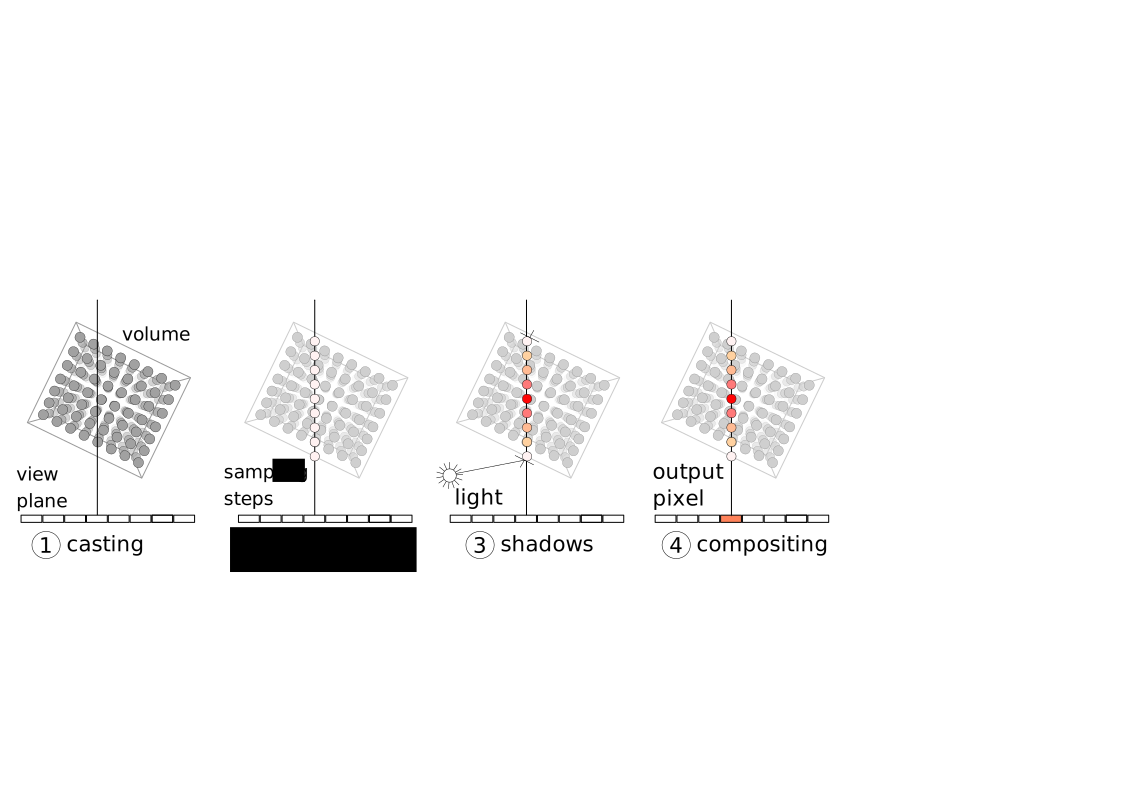
\includegraphics[scale=.68]{images/raycasting-steps.png}
\caption{Volume ray casting decomposed steps.}
\label{fig:raycastingsteps}
\end{figure}

Therefore, in order to be able to traverse the volumetric data, as the first phase of the proceed of the algorithm, it is necessary to compute the entry and the exit point, in the 3-Dimensional space, of each ray with respect to the position of the volume with respect to the world-space coordinates. %ref to word-space coordinates%
These exit and entry point, as will be described in the implementation chapter of this work, requires some collision detection calculation. 
\linespace

The second step involves the sampling of the voxels inside the volume and this operation is performed at a constant step along the ray, as shown in Figure \ref{fig:raycastingsteps}.2.

Color and opacity are sampled from the volume data in order to compute the final output view image and these values are sampled as emission values stored into the voxels, usually in the range of a 8 bit gray scale, from 0 to 255.
\linespace

The next phase involves spending few more computational power in order to calculate a properly shadowed value of the color, from the previous step (Figure \ref{fig:raycastingsteps}.3). This is a very fundamental part of the proceed in the medical imaging context as it allows a good, otherwise useless, visualization of the dataset.

In order to achieve the needed fine looking result, different approach can be taken involving some volumetric shading technique to approximate the light integral, such as Blinn-Phong global illumination model and approximation algorithm.
\linespace

In the end, the final result is store into a 2-Dimensional image by means of compositing all the values sampled and transformed during the previous steps, into one single value per pixel,as shown in Figure \ref{fig:raycastingsteps}.4.

Usually such values are store as vectors that belongs to the RGB color space%ref to rgb chapter%
however as already seen in the color space chapter there exists different and more appropriate color space that doesn't encode the illumination inside the color itself.
\linespace

In order to compose such values there exists different operators that can be applied. The most common one is the over operator proposed by Porter%cite porter
because it is also capable of dealing and preserving semi-transparency voxels values according to their opacity. More of these operators are describe in the Composition schemas section.
\linespace

There are two ways of compositing, back-to-front and front-to-back. They both have their pros and cons: back-to-front is the most simple method, however it is also the most expensive one in terms of computational requirements,because it doesn't allows any kind of optimization as all the voxels, from the least visible to the closest and visible one, must be accounted.
On the other hand, front-to-back method requires more storage memory as additional variable are needed to save characteristics such as transparency.
\linespace

The volume ray casting technique proceed can be summarize as follows:
\begin{enumerate}
\item Define the number of ray according to the view screen size.
\item Before casting, compute the starting and exiting point as 3-Dimensional coordinates with respect to volume world-space position.
\item For each pixel of the view screen cast a ray through the volumetric data set.
\item At a constant step, sample voxels values of color and opacity and store them into the respective ray.
\item Transform each of these value by means of volumetric shading technique
\item Compose the final result back-to-front or front-to-back applying a chosen operator.
\end{enumerate}

Ray casting has different advantages, as it is simple and easy to implement in its very basic version, it allows different degrees of freedom in choosing which method or algorithm should be used during the different phases and its final result doesn't suffer of any artefacts that are present with other techniques instead.

However, there is a major cons while using this technique: its basic implementation is very slow and poor in terms of efficiency. This problem is the reason why it is not yet used in state-of-the-art medical imaging techniques even  it does produces very good results.
\linespace

The aim of this work, as already stated, is exactly to build starting from scratch, a volume ray casting algorithm that can compete with nowadays state-of-the-art competitors exploiting modern graphics devices.

\subsubsection{Composition schemes}
%rifrasare
In this section the different number of composition schemes will be described and explained for the sake of completeness. that are used during the process of direct volume rendering and especially fundamental for the volume ray casting technique.

There exists a number of different composition schemes that can be used:
\begin{itemize}
\item Maximum intensity projection (MIP)
\item First hit
\item Accumulate
\item Average
\end{itemize}  
%inserire immagine
All of the above treat the sampled value of the voxel in different way. However they are used to extract the isosurfaces and to render them. There are not advantages or disadvantages on using one method or the other, because they are used to archive different results in terms of final image.
\paragraph{Maximum intensity projection} Maximum intensity projection is often used for magnetic resonance angiograms or to extract vessel structures from CT or MRT scans. For rendering, it uses the greatest value sampled from the ray and the final result can be seen in the Figure. 

%add image
\paragraph{First hit} First hit composite method works by means of using the sampled scalar value that is higher that a defined threshold limit. Then, the isosurface is extracted and rendered.

\paragraph{Accumulate} Accumulate compositing method is similar to the over operator. It works accumulating the intensity Color until enough opacity is collected. The final result will shown also transparent layer whom opacity is above 0 and 
therefore still visible.

\paragraph{Average} Average produces essentially the same picture of X-ray. Additionally, it does not take into account any opacity value.

\subsection{Volume rendering state-of-the-art} 
%TODO scrivere una migliore introduzione pro 500 e pro 1000

In this section volume rendering techniques proceed and characteristics whom are used in state-of-the-art algorithms and systems deployed for rendering and creating interactive images of objects and phenomena represented as 3-Dimensional data,within the context of medical imaging and scientific visualization in general. 

Nowadays there exists different implementation of the previously described techniques that stands out in terms of output image quality in volume rendering. However, it is not only about high efficient software implementation, but also tangible hardware that is built to let the software part perfectly fits on and reach the best results.
\linespace

The first system worth mentioning is VolumePro 500, built by Mitsubishi Electric company in 1999 based on the already existing architecture known as Cube-4. The system exploit the power capability of the shear-warping techniques with standard factorization to archive rendering of $256^3$ renders or smaller volumes at 30 frames per second.%TODO add ref 87,87


The system was subsequently acquired by TeraRecon Inc. which improved it and then release the VolumePro 1000 system. This enchanted version is a single chip for real-time volume rendering capable of processing volume data at a rate of $10^9$ samples per second, using a novel technique called Shear-Image order ray casting, that inherits the ray-per-pixel casting method of image-based ray casting technique, but introduces a new intermediate sample space in which the axes are sheared with respect to the image place(hence the name shear-image order). 
\linespace

Both systems deploys a highly optimized memory address interface that enables efficiently read blocks and axis-aligned slices of voxels without wasting any more storage space.%TODO add ref 131
For the sake of clarity VolumePro 500 will not be discussed, instead a description of his successor VolumePro 1000 will be given along with its adopted approach, as they can be of much more interest for the readers and also because as the latter is the result of improvements of the first one, it is a better candidate to represent state-of-the-art implement in the direct volume rendering category. 


%Another technology currently deployed as state-of-the-art volume rendering and real-time visualization is based on the well known Marching cubes technique and it is called VESTA. It belongs to 
%TODO search something about VESTA for surface exctracting algorithm
\paragraph{VolumePro 1000} Volume Pro 1000 is developed and improved by TeraRecons Inc. which released the first version of the system in 2002.TeraRecons release is the successor of Volume Pro 500 which was built  the company Mitsubishi Electric and release it in 1999, improving an already existing architecture known as Cube-4, developed at SUNY Stony Brook.
\linespace

The VolumePro 1000 system %TODO 131
uses a novel shear-image order ray-casting approach (Figure \ref{fig:shearimageorder}). %TODO ref visualization handbook 247
 Firstly, Volume Pro architecture deploy a special memory address arithmetic known as 3D skewing, as already said, let the system save storage memory. 
\linespace

The core idea is to casts rays directly through centers of pixels, as standard ray casting technique. However, it keeps the set of slices aligned to the base plane, very similar to 2D texture method. The 3D viewing transformation, or affine transformation, used as part of the base concept is decomposed in two different explicit matrices: one that transform from voxel coordinates space to an intermediate coordinate system called sample space; the second one that transform the depth values of the sampled points to reflect their distance from the image plane. %TODO pag 248 vis handbook

\begin{figure}[hbtp]
\centering
\includegraphics[scale=0.3]{images/shear-image-order.png}
\caption{Shear-image order ray-casting. Grey samples are interpolated between original volume slices.}
\label{fig:shearimageorder}
\end{figure}


These two transformation enables Volume Pro 1000 to produce final images that does not have to be warped because they are already aligned along viewing rays from image-plane pixels, eliminating the intermediate and the final shearing operations required by standard shear-warp technique. 

Therefore it produces images that are of higher quality than the ones produced by traditional shear-warping, like the one used in VolumePro 500 instead. %show figure 11.17
\linespace

As well as it predecessor VolumePro 500, it performs a triliniear interpolation of the volume data and computes the gradient vector in hardware to prevent undersampling and artifacts popping out. It does so also reconnecting to the work of Rezk-Salama on 2D texture slicing, as it is possible to generate additional interpolated slices between original voxel an shift them with sub-pixel accuracy, artifacts keeping, in this way, ray and sample spacing constant. %TODO cire handbook


Another aspect that characterize VolumePro 1000 system is that Voxels can have up to four fields, each of them is associated with a lookup table. Those are organized in a set and used during the classification phase; they can be combined by means of a hierarchy of arithmetic-logic units as they are built in cascade.
\linespace

The shear image proceed can be divided in two parts: The first part operates like the standard shear-warp technique by stepping through one slice of the volume at a time, that is stored in the main memory. Then, it interpolates adjacent voxel slices to obtain new slices called z-interpolated samples. 

These resulting slices will appear to be organized in a grid parallel to the x and y dimensions of the volume, as no other interpolation took place before.
\linespace

The second part, traverse each of the new generate slice of z-interpolated sampled value. It enumerates the sample point on the rays that intersect with the slice and it computes the color and the opacity value of each one of the z-interpolated samples. It also associate a depth values to measure the distance from the sample to the eye and are used to embed polygons in the rendered images.


Finally those computed values are accumulated along the respective rays and a rendering of the volume is produced and stored directly on the image plane.
\linespace

As shading technique, in VolumePro 1000  Phong shading illumination model is used, trying to ensure a correct gradient, and Compositing is made by means of alpha blending maximum intensity projection like  VolumePro 500, but its hardware also supports early ray termination that let it increase  its performance.

\linespace
Part of this work is to be able to built a fully image-based algorithm based on the ray casting technique which reaches the degree of efficiency and quality in term of execution speed and output image quality similar to the ones reached when deploying VolumePro 1000. In the next section a fully detailed description of the architecture, technologies and concepts used in an attempt to reach such results.
\pagebreak
\section{Renderer implementation} 
This work focuses on building a volume rendering algorithm that can exploit the power available on graphics hardware, through parallelization. Furthermore, the objective is to distribute such algorithm in an environment that is regularly used in research and academic fields, in order to simply the integration in other systems whom need an efficient volume renderer.


In this chapter, will be given a description of technologies used, and reasons behind each made choice, to be able to fulfil the thesis objectives.
\linespace

First of all, an explanation about MATLAB environment and its precious MEX functions: what are they, why are they useful and how, in order to integrate a common MATLAB program with one written in an external programming language like C++.

Then, a brief introduction over CUDA framework and programming model, why it has been chosen over other parallel programming libraries and framework and how it works.

After the technologies section, there will be a deep dive into the algorithm itself; describing the underlying architecture on which it is modelled and the concepts borrowed from the original work by Levoy, on efficient volume ray tracing algorithm.
\linespace

There will be a first section about the base non-parallel version of the developed algorithm, which has been built first for different reasons:

First of all, the non accelerated algorithm has been developed in order to have a lower bound in terms of efficacy and efficiency of the renderer; very useful, as it will be used during comparisons and while drawing the final conclusions about this work.

Secondly, a natural way of developing parallel software is to start from the non-parallel counterpart and then proceed step by step with a conversion from the linear execution and written code, to the concurrent execution and respective instructions.

A full explanation of the different parts that are composing the algorithm will be given along with excerpts of the code, trying to separate each concept following the steps describe in the previous section about direct volume rendering technique with respect to ray casting.

The integration between the MATLAB environment and the C++ code will be describe focusing on single instructions needed to communicate from and to a MATLAB program.
\linespace

Then, the accelerated version will be presented and explained. A description of the proceed need to go from the basic version to the parallel one will be given, which shows the code transformations from the common programming model used for the basic version to the CUDA programming model. 

Description of the most crucial code part will be given that shows those transformations along whit whichever changes in underlying data structure involved.

\subsection{Technologies} 
\subsubsection{MATLAB and MEX functions}
MATLAB, that stands for matrix laboratory, is a multi-paradigm numerical computing environment and proprietary programming language developed by MathWorks. It allows matrix manipulation, easy plotting of data and function and creation of user interface.
It is an integrated development environment which widely use in academic field, due to its power and enormous number of functionality that are available with the core version but whom rocket-up exponentially with the numerous plug-ins.

A MATLAB application is built using the MATLAB scripting language and the Command Window is usually used as an interactive mathematical shell or to execute MATLAB code.
%ref https://en.wikipedia.org/wiki/MATLAB
\linespace

One of the most interesting and useful feature of MATLAB, with respect to this work, is the MEX file.
\paragraph{MEX file and functions} The term MEX stands for "MATLAB executable". %ref https://de.mathworks.com/help/matlab/matlab_external/introducing-mex-files.html
There are different definitions:
\begin{itemize}
\item MEX file: it refers to the source code file written in an external programming language such as C, C++ or Fortran,
\item MEX function: it refers to the binary subroutine compiled from the source code file.
\end{itemize}

A MEX file can contain only one function or subroutine which is identified by the file name without the file extension.

MEX functions have very important features such as:
\begin{itemize}
\item They can be dynamically loaded inside a MATLAB program as normal MATLAB functions
\item They are compiled at runtime.
\item it exposes different API that allows the integration of external function simplifying the communication between the workspace and the subroutine.
\end{itemize}

In order to be able to create a MEX file and therefore call MEX functions from MATLAB a MATLAB-supported compiler must be installed such as: MinGW or MS C++\footnote{https://de.mathworks.com/support/requirements/supported-compilers.html} and write the function with one the available API. For the sake of simplicity, only APIs used for this thesis will be explained which are used for functions written in C or C++ programming languages, called C MEX API and C Matrix API.

The first step to write a MEX function in C++ is to define it with \textit{mexFunction} function, which is the entry point to C/C++. It acts as the gateway between C++ and MATLAB workspace that identify a MEX function.

When a MEX functions is invoked, MATLAB find and loads the corresponding MEX functions of the same name. Then it searches for a symbol named \textit{mexFunction} within the MEX function. Such function is defined as follows: %ref https://de.mathworks.com/help/matlab/apiref/mexfunction.html

\begin{cpp}[caption={MEX functions C/C++ entry point definition},label=code:mexfunction]
#include "mex.h"
void mexFunction(int nlhs, mxArray *plhs[], int nrhs, 
	const mxArray *prhs[])
\end{cpp}

The signature that define this function is composed of four arguments, which are automatically seeded by MATLAB when the MEX function is called with the calling arguments.

The arguments \textit{nlhs} and \textit{nlhs} contains the number of right and left arguments, respectively. Therefore, it is clear that \textit{plhs} and \textit{prhs} are two pointers to arrays of type mxArray, with length of \textit{nlhs} and \textit{nrhs}. These pointers are the input arguments and the outputs of the MEX function respectively, which has the following general form, in the MATLAB syntax.

\[
\begin{matrix}
o_{0},o_{1},o_{2}, \cdots
\end{matrix}
= func (a_{0}, a{1},a{2}, \cdots )
\]

Where $o_{m}$ represents the $m-element$ left-side output argument and $a_{n}$ represents the $n-element$ right-side input argument, with $n < prhs$ and $m < plhs$,respectively.
\linespace

The fundamental type underlying MATLAB data is \textit{mxArray}. It is an opaque C data type\footnote{An language type is defined \textit{opaque} when the concrete representation of the type is hidden from its users, and the visible implementation is incomplete. This enforces information hiding, since its values can only be manipulated by calling help functions that have access to the missing information.} and the structure contains the following information about the array:

\begin{itemize}
\item Its type
\item Its dimensions
\item The data associated with the array
\item If numeric, whether the variables is real or complex
\item If sparse, its indices and non-zero maximum elements
\item If a structure or object, the number of fields and filed names
\end{itemize}
\linespace

All MATLAB variables (including scarlas, vectors, matrices, character arrays, cell arrays, structures or objects) are stored as MATLAB arrays, whom are declared of type mxArray in C/C++.

There exists different data types in MATLAB:
\paragraph{Complex double-precision matrices}
Complex double-precision matrix is the most common data type in MATLAB. These matrices are of type \textit{double} and have dimensions m-by-n, where $m$ and $n$ are the number of rows and the number of columns, respectively. The data inside the matrix is stored as a vector of interleaved, double-precision numbers where the real and the imaginary parts are stored next to each other\footnote{To test for a non complex matrix, mxIsComplex helper function must be called.}.
\paragraph{Other numeric matrices}
MATLAB also suppers single-precision floating point and 8, 16, 32 and 64-bit integers, both signed and unsigned.
\paragraph{MATLAB char arrays}
In MATLAB, \textit{char} arrays are data stored as unsigned 16-bit integers. In order to convert a MATLAB \textit{char} array to a C-style string, \textit{mxArrayToString} subroutine bust be called; vice versa, to convert a C-Style string to a \textit{char array}, \textit{mxCreateString} is used.
\paragraph{Cell arrays}
Cell arrays are a collection of MATLAB arrays where each \textit{mxArray} is referred to as a cell. Cell arrays allow storing together MATLAB arrays of different types. They are stored in a similar manner to numeric matrices, except the data portion contains a single vector of pointers to \textit{mxArrays}. Member of this vector are called cells and each cell can be of any supported data type, even another cell array.
\paragraph{Structures}
Structures are stored in the same way as a 1-by-n cell array where $n$ is the number of fields in the structure. Members of the data vector are called fields and each filed is associated with an identifying name, stored in the \textit{mxArray}.
\paragraph{Objects}
Objects are stored and accessed the same way as structures. In MATLAB, objects are named structures with registered methods; Outside of it, an object is a structure that contains additional stored information of the class name, that identify the name of the object.
\paragraph{Multidimensional arrays}
MATLAB arrays of any type can be multidimensional. A vector of integers is stored where each element is the size of the corresponding dimension. the storage method of the data is the same as for matrices.
\paragraph{Empty arrays}
In MATLAB, arrays of any type can be empty. An empty \textit{mxArray} is one with at least one dimension equal to zero.\footnote{For example, a double-precision \textit{mxArray} of type double, where its dimensions $m$ and $n$ are equal to 0 and the pointer is NULL, is an empty array.} 
%ref https://de.mathworks.com/help/matlab/matlab_external/matlab-data.html
\linespace

In order to declare a data structure of type \textit{mxArray} inside C/C++ code and to define its values, the following statement must be written:
\begin{cpp}[caption={Declaration and definition of a floating-point non complex mxArray named myData of size m-by-1, initialized to 0},label=code:createmydata] 
mxArray *myData = mxCreateDoubleMatrix(m,1,mxREAL);
\end{cpp}

There exists an mxCreate* function for each of the supported MATALAB data type other than double-precision floating-point array, for example\footnote{For the sake of clarity some creational functions are omitted. The full list of available functions can be found at \cite{create_del_mxarray:2}} 
\begin{itemize}
\item \textit{*DoubleScalar}: for Scalar, double-precision array.
\item \textit{*NumericMatrix}: for numeric matrix of size m-by-n.
\item \textit{*String}: for 1-by-n array initialized to a specified string.
\item \textit{*LogicalMatrix}: for m-by-n logical array.
\item \textit{*StructMatrix}: for m-by-n structure array.
\item \textit{*CellMatrix}: for m-by-n cell array
\end{itemize}

The creation counterpart is defined as the following statement, that frees the dynamic memory allocate by mxCreate* functions such as the previous call:

\begin{cpp}[caption={Deallocation of dynamic memory referred by myData \textit{mxArray} pointer, from Listing \ref{code:createmydata}},label=code:mxarraydestroy]
mxDestroyArray(myData);
\end{cpp}

\textit{mxDestroyArray} deallocates memory for the specified \textit{mxArray} including:
\begin{itemize}
\item Characteristics field of the \textit{mxArray} such as size and type.
\item Associated data arrays
\item Fields of structure arrays
\item Cells of cell arrays
\end{itemize}

However, it should not be called on a \textit{mxArray} that:
\begin{itemize}
\item It is returned in a left-side argument of a MEX function.
\item Returned by the \textit{mxGetField} or \textit{mxGetFieldByNumber} functions.
\item Return by the \textit{mxGetCell} function.
\end{itemize}
%ref https://de.mathworks.com/help/matlab/apiref/mxdestroyarray.html

The last bit about MEX functions and \textit{mxArray} fundamental type is how to access and write data from and to an defined \textit{mxArray}.

First of all, as already mentioned, any variable declared as a \textit{mxArray} is indeed and array in C/C++ context. Therefore as any other array in C/C++ the array subscript operator [ ] is defined, that allows users to access the element stored at the position, specified by an integer value. %ref http://www.cplusplus.com/doc/tutorial/arrays/
\linespace

In the same way helper functions were defined to create new \textit{mxArrays}, helper functions are defined to access and write data with respect to the MATLAB target type.

For example, the following statement describe how to read from the MEX function input argument \textit{prhs} element at position 0 which points to an array of one single element.

\begin{cpp}[caption={Accessing the first non-imaginary element of the mxArray pointer passed as argument from the MEX function input arguments},label=code:mxarraygetscalar]
/* get the value of the scalar input  */
double multiplier = mxGetScalar(prhs[0]);
\end{cpp}

The array subscript operator works the same manner as in C/C++, then it can be used to modify and set values at specified array position. Listing \ref{code:mxarrayset} shows how to create a new mxArray matrix of floating-point non-complex type of size m-by-n and how to set a new value for first element of the first output argument of the MEX function.

\begin{cpp}[caption={Create the output matrix corresponding to the first output array. Get the pointer to the real data and set a new value for the first element},label=code:mxarrayset]
/* create the output matrix */
plhs[0] = mxCreateDoubleMatrix(m,n,mxREAL);
/* get a pointer to the real data in the output matrix */
double *outMatrix = mxGetDoubles(plhs[0]);
/* modify the first element with a new value */
outMatrix[0] = 1;
\end{cpp}

As can be seen, the notation used was with a single couple of square brackets, even if the output matrix is of size m-by-n. The reason is that, matrices defined of type \textit{mxArray} are accessed by means of a single index, because of the way C/C++ storing technique allocate matrix in a contiguous fashion, in row-major order\footnote{In a row-major order, the consecutive elements of a row are allocated in memory next to each other. %ref https://en.wikipedia.org/wiki/Row-_and_column-major_order
}.


\subsubsection{CUDA framework}
CUDA is a framework and programming model that let its users build parallel applications which exploit the power of GPUs, developed by NVIDIA whose objective was to release a \textit{bundle} which consists of a compiler, libraries, and runtime software, to enable programmers to readily access a new data-parallel computation model and develop application.\cite{KirkHwu_2014:3}

The computing system, from the CUDA perspective, is divided in two main parts: an host and one or more devices. The host is a traditional CPU, and a device is a processors with a massive number of arithmetic units, typically a GPU.

In order to be able to safely perform parallel computation, a modern software application must at least exhibit what is called data parallelism.\footnote{Data parallelism in snot the only type of parallelism widely used in parallel programming. Task parallelism has also been used extensively in parallel programming. Task parallelism is typically exposed through task decomposition of applications.\cite{KirkHwu_2014:3}}

Such phenomenon allows arithmetic operations to be performed on different parts of the data structure in parallel, and CUDA devices accelerate the executions of these applications by applying their massive number of arithmetic units to these data-parallel programs.
\linespace

CUDA is heterogeneous programming model because any CUDA program reflect the coexistence of a host(CPU) and one or more devices(GPUs) in the computer. Indeed, a CUDA source file usually have a mixture of both host and device code.
Any traditional C/C++ program can be seen as a CUDA program that contains only host code.

\begin{cpp}[caption={CUDA keywords for function declarations},label=code:cudakeywords]
/*Marked function that will be executed on the device, but only 
	callable from another device function*/
__device__ float deviceFunction()

/*Marked function that will be executed on the device, but only 
	callable from a host function*/
__global__ void kernelFunction()

/*Marked function that will be executed on the host that can be 
	called only from another host function*/
__host__ float hostFunctions()
\end{cpp}


Host and device code are clearly marked with special CUDA keywords, as shown in Listing \ref{code:cudakeywords}. $\_\_device\_\_$ and $\_\_global\_\_$ keywords mark functions that will run on the processing unit of connected devices. The subtle difference resides on who can call such functions, $\_\_device\_\_$ marked functions are called from another functions that runs on the device, and $\_\_global\_\_$ marked ones are called only from host-running functions. 
\linespace

The $\_\_host\_\_$ keyword indicates that the functions being declared is an host function. Such function is simply a traditional C/C++ function that execute on the host and can only be called from another host function. By default, all functions that are not marked by any CUDA keywords, are host functions.It is interesting noting that it is possible to use both $\_\_host\_\_$ and $\_\_device\_\_$ keywords in a function declaration, as it instruct the compilation system to generate two versions of the same function, one executed on the host and one execute on the device.
\linespace

$\_\_global\_\_$ marked device functions are also known as \textit{kernels}. When a kernel function is called, or \textit{launched} from an host call, it is executed by a large number of threads on a device to exploit data parallelism, generated by the CUDA runtime system.

All threads that are generated by a kernel launch are collectively called a \textit{grid}. Each grid is organized into an array of thread blocks.

Such blocks of a grid are of the same size and each block can contain up to 1024 thread. Figure \ref{fig:cudagridblock} shows how threads hierarchy is organized, where each block consists of 256 threads.
\begin{figure}[hbtp]
\centering
\includegraphics[scale=0.7]{images/cudathreadgrid.png}
\caption{All threads in a grid execute the same kernel code and are organized into an array of thread blocks.}
\label{fig:cudagridblock}
\end{figure}


Each thread in a block has a unique $theadIdx$ index,similarly each block in a grid has a unique $blockIdx$ identifier. This allows each thread to be uniquely identified inside a grid by combining its $threadIdx$ and the $blockIdx$ values to along with the specified block's number of thread values $blockDim$, as described by the following formula:

\[
i = blockIdx.x * blockDim.x + threadIdx.x
\]

By launching the kernel with a larger number of blocks, one can process larger amount of data. For example, by launching a kernel with $n$ or more threads, it is possible to process vectors of length $n$.
\linespace

In order to launch a kernel function, the host code has to set the frid and thread block dimensions via \textit{execution configuration} parameters, illustrated in Listing \ref{code:kernelconfig}.

The configuration parameters are given between the $<<<$ and $>>>$ before the traditional function arguments. The first configuration parameter gives the number of thread blocks in the grid. The second one specifies the number of threads in each thread block. In the example below, there are 256 threads in each block and $n/256.0$ thread blocks where $n$ is the dimension of our data.

\begin{cpp}[caption={A kernel function launch statement.},label=code:kernelconfig]
kernelFunc<<<ceil(n/256.0), 256>>(input data);
\end{cpp}

Once device functions and data declarations are added into a C/C++ source file, it is no longer acceptable to a traditional compiler. The code needs to be compiled by a compiler that recognizes and understands these additional declarations. For this reasons, a CUDA compiler by NVIDIA is used, called NVCC.
Figure \ref{fig:cudacompiler}, shown the NVCC that processes a CUDA program at the top, suing the CUDA ketwords to separate the host code from the the device code. The host code is further compiled with the hots's standard C/C++ compilers and in run as a traditional CPU process.Instead, the device code is further compiled by a runtime component of NVCC and execute on a GPU device.
\begin{figure}[hbtp]
\centering
\includegraphics[scale=0.7]{images/cuda-compiler.png}
\caption{Overview of the compilation process of a CUDA program}
\label{fig:cudacompiler}
\end{figure}

%TODO add conclusion


\subsection{Architecture} 
This work and actual implementation follows the previous work of Levoy about volume ray tracing, mainly.

Figure \ref{fig:architecture} shows the algorithm architecture with respect to the entire ecosystem and how it interact with other MATLAB programs as well as the relationship with the accelerating CUDA framework. As can be seen, in order to build a broadly available rendering algorithm all the proceed is encapsulated inside a MEX function that will let users to include it inside every other MATLAB program that require a fast effective and real-time volume rendering algorithm, by passing the right required arguments and receiving the resulting output 2-Dimensional image with the projected volumetric input dataset as expected from a volume ray casting algorithm.\cite{levoy_1988:4}

\begin{figure}[hbtp]
\centering
\includegraphics[scale=0.6]{images/volumearchitecture.png}
\caption{Algorithm architecture. A MATLAB program calling with input arguments the MEX function that return the final output image}
\label{fig:architecture}
\end{figure}

The procedure as other MEX functions, is called by the file name as showed in Listing \ref{code:volumecall}. It requires different input arguments to be able to work properly :
\begin{itemize}
\item Two volumetric datasets, containing different information,the second one optional.
\item The 3-Dimensional size of the volume.
\item Rotation components, defined as Yaw, Pitch and Roll.
\item Alpha opacity values defined as an array of double.
\item Array of colors, defined in RGB format.
\item The specular component, that defines the ratio between a full diffuse rendering and an full specular. 
\item The threshold value, used to select which voxel intensity is discarded.
\end{itemize}

\begin{cpp}[caption={Volume rendering MEX function call with left and right arguments, respectively output and input arguments},label=code:volumecall]
output = Volume(vol,objs,infoStruct);
\end{cpp}

The first volumetric dataset store the voxels' intensity values that defined the actual volume. Each value is bounded to $[0,\,255]$ value range, where $0$ is the empty space around the volume. The second volume stores the different objects that are composing the original volume. Values are stored in the same way as in the original volume, as a 3-Dimensional grid of voxels but instead of intensity they represent objects. 

The data format is of type integer in the range of $[0,\,(N-1)]$ where $N$ is the total number of objects whom compose the volume. This second volume is optional but it can't be omitted from the input arguments, so it can be passed as empty volume.

Except the two volume datasets, all the other arguments must be defined as a MATLAB struct, as it requires a lot of arguments.
\linespace

The threshold value let users display all voxels with intensity value greater or equal then the threshold, as stated in \cite{levoy_1988:4} this produces 3D regions of opaque voxels, where the outermost layer of which is the desired surface.
The classification procedure employed is this work wouldn't be able to display concentric semitransparent surfaces or object, as reported by Levoy in \cite{levoy_1988:4}. To solve this issue, the second volumetric dataset that contains every object of interest in the volume is used along with the opacities array.
\linespace

The alpha opacities array is used to define the opacities of the object. Indeed, the size of the array $N$ must be equal to the number of objects defined in the second volume. 
Although, this array have also another purpose, if the size $N$ is equal to 1 it defines the global opacity of the volume.

Another input argument strictly related to the classification and number of objects defined in the second volume, is the colour array.
\linespace

The colour array helps the visualization separating all the objects with different colours. The colours must be defined in RGB color space and format.
As well as for the opacities array, the colours array size $N$ must be equal to the number of objects defined in the visualization. The only little difference between the behaviour of the algorithm for opacities and colours is that if no colour is defined in input and no objects are stated as well, the algorithm will render the volume in a gray scale using directly voxels intensity values. 
\linespace

The last argument is the rotational array in Yaw, Pitch and Roll format. In order to build an interactive system on top the algorithm of this work, a camera is needed to let users interact with volume and look at it from different point of view. Therefore, the rotation array allows moving such camera around the center of volume by means of the definition of a Yaw angle, a Pitch angle and a Roll angle that allow a camera to move freely around a pivot point.
\linespace

Very similar to the way Levoy formalized his work and as explained previously in direct volume rendering techniques section,
Figure \ref{fig:steps} shows how the algorithm has been decomposed in different steps. Each step has been developed almost independently while trying to apply the most effective techniques.


\begin{figure}[hbtp]
\centering
\includegraphics[scale=0.5]{images/steps.png}
\caption{Algorithm expanded steps whom cover different important aspects.}
\label{fig:steps}
\end{figure}

\subsection{Basic volume ray casting} 
In this section, the proceed steps showed before will be explained step-by-step describing all the techniques employed in each step in order to reach the goal behind this work.
Starting right after reading the input volume and the other input arguments the first step is to set up the bounding box around the volume.

\paragraph{Bounding box}

A bounding box, also known as \textit{minimum bounding box} in geometry, is a box for a point set $S$ in $N$ dimensions with the smallest measure within which all the points lie, and it is usually used to speed up computations. In the 2-Dimensional case it is called the \textit{minimum bounding rectangle} and the measure used to check the required condition is the area. In the 3-Dimensional case instead the measure used of the bounding box is the volume.
%TODO cite https://en.wikipedia.org/wiki/Minimum_bounding_box
\linespace

There exists two different type of bounding box (Figure \ref{fig:boundingbox}): \textit{Axis-aligned minimum bounding box} and \textit{Arbitrarily oriented minimum bounding box}.

\begin{figure}[hbtp]
\centering
\includegraphics[scale=0.7]{images/boundingbox.png}
\caption{Axis-aligned(left) and Arbitrarily oriented(right) minimum bounding boxes coloured in gray.}
\label{fig:boundingbox}
\end{figure}


\textit{Axis-aligned minimum bounding box} or \textbf{AABB} for a given point set is its minimum bounding box subject to the constraint that the edges of the box are parallel to the coordinate axes. It used to approximate location of an object in question and as a very simple descriptor of its shape.

\textit{Arbitrarily oriented minimum bounding box} instead is the minimum bounding box, calculated subject to no constraints as to the orientation of the result.
\linespace

The AABB bounding box concept in 3-Dimension and in computer graphics, as well as in this work is known under the name of \textit{bounding volume}. It is used to improve the efficiency of geometrical operations by using simple volume to contain more complex objects, as simpler volumes have simpler ways to test for overlap.
%TODO cite https://en.wikipedia.org/wiki/Bounding_volume

In ray casting, and so in this implementation as well, bounding volumes are used in ray-intersection test. If the ray does not intersect the bounding volume, it cannot intersect the object contained within, allowing trivial rejection. Listing \ref{code:gridclass} shows the Grid class that represent the axis-aligned minimum bounding box and the member function \textit{isInsideGrid} that checks the condition if a given triple of indices falls inside the volume boundaries.

\begin{cpp}[caption={Grid class definition.},label=code:gridclass]
class Grid {
public:
	Vector3 bounds[2] = { 0 };
	Grid(const Vector3 &min, const Vector3 &max) 
	{
		bounds[0] = min, bounds[1] = max;
	}
	inline
	bool isInsideGrid(const int&i, const int&j, const int&k) 
	{
		return 
			i > bounds[0].x && 
			j > bounds[0].y && 
			k > bounds[0].z && 
			i < bounds[1].x - 1 &&
			j < bounds[1].y - 1 && 
			k < bounds[1].z - 1;
	}
	friend 
	std::ostream& operator<<(std::ostream&s, const Grid&g)
	{@ $\cdots$ @}
};
\end{cpp}

This is one of the first speed-up in the implementation as part of the sequent ray casting and voxels intersections step of the algorithm. The reason is that with \textit{AABB} bounding volume all the multitude of cast rays can trivially checked if they end up inside or outside of volumetric dataset boundaries.
\linespace

Listing \ref{code:gridinit} shows how the bounding box is initialized with respect to the size of the volumetric dataset by means of the \textit{Grid} class, where the first parameter \textit{Vector3(0)} is the origin of the world space and \textit{sizeArray} is the array that stores the volume dimensions and th

\begin{cpp}[caption={Grid object initialization.},label=code:gridinit]
Grid grid(Vector3(0), 
	Vector3(sizeArray[0], sizeArray[1], sizeArray[2])
	);
\end{cpp}

\paragraph{Camera setup} The next step is set the camera parameters. The meaning of the camera is to allow users to interact with the volume performing rotation around the center of the dataset.

First the class representing the camera must be defined. Listing \ref{code:cameraone} shows the attributes that compose the class, its constructor and methods headers, which will explained later on.

\begin{cpp}[caption={Camera class definition with },label=code:cameraone]
class Camera {
public:
	Vector3 center;
	Vector3 from,to,forward,backward,right,up;
	Matrix4x4 lookAt,rotationM;
	double theta, phi, sigma;

	Camera(Vector3 from, Vector3 to) {
		this->from = from;
		this->to = to;
		this->rotationM = Matrix4x4();
	}
	void yaw(const double& angle) {@ $\cdots$ @}
	void pitch(const double& angle) {@ $\cdots$ @}
	void roll(const double& angle) {@ $\cdots$ @}
	void setupLookAtMatrix() {@ $\cdots$ @}
};
\end{cpp}

As can be seen, the Camera class constructor require in its signature two 3-Dimensional vectors. These two vectors are needed in order to build the \textit{lookAt} matrix that let users position and steer the camera. The \textit{from} vector defines the position of the camera in the 3-Dimensional world space, while the second one, the \textit{to} vector, defines the camera orientation with respect to a target point which the camera will be pointing at.
The last statement in the constructor initialize the transformation matrix that will hold all the subsequent rotation matrices which will be created by the yaw, pitch and roll functions.
\linespace

Therefore, the camera will be defined and initialized as shown in Listing \ref{code:camerainit}, where \textit{sizeArray} is still the array that stores the volume dimensions and \textit{options.viewOffest} is a constant double precision variable that defines a viewing offset that let the camera be positioned not too far from the volume but enough to be able to show the entire volume.

\begin{cpp}[caption={Camera definition and initialization.},label=code:camerainit]
Camera camera(
	Vector3(sizeArray[0]/2 + options.viewOffset, 
		sizeArray[1]/2, sizeArray[2]/2), 
	Vector3(sizeArray[0]/2, sizeArray[1]/2, sizeArray[2]/2)
	);
\end{cpp} 

Yaw, pitch and roll functions create the transformation matrices, as defined in the section about affine transformations, that rotate the camera. As already said, those transformation are needed to let the camera move around a pivot point, which is the center of the volume as defined in the construction call.

Listing \ref{code:camerarotate} shows the yaw, pitch and roll rotations, that are respectively Z-Axis, Y-Axis and X-Axis in the world space.

\begin{cpp}[caption={},label=code:camerarotate]
void yaw(const double& angle) { // z-axis
	theta = degToRad(std::fmod(angle, 360));
	Matrix4x4 rZ = Matrix4x4(
		std::cos(theta), -1*std::sin(theta), 0, 0,
		std::sin(theta), std::cos(theta), 0, 0,
		0, 0, 1, 0,
		0, 0, 0, 1);
	rotationM = rotationM.matrixMulti(rZ);
}
void pitch(const double& angle) { // y-axis
	phi = degToRad(std::fmod(angle, 360));
	Matrix4x4 rY = Matrix4x4(
		std::cos(phi), 0, -1*std::sin(phi), 0,
		0, 1, 0, 0,
		std::sin(phi), 0, std::cos(phi), 0,
		0, 0, 0, 1);
	rotationM = rotationM.matrixMulti(rY);
}
void roll(const double& angle) { // x-axis
	sigma = degToRad(std::fmod(angle, 360));
	Matrix4x4 rX = Matrix4x4(
		1, 0, 0, 0,
		0, std::cos(theta), -1*std::sin(theta), 0,
		0, std::sin(theta), std::cos(theta), 0,
		0, 0, 0, 1);
	rotationM = rotationM.matrixMulti(rX);
}
\end{cpp}

Each function has an input argument that is the rotating angle expressed in degrees of the respective rotational axis. This angle in then converted from degrees to radiant due to the formal requirement of the mathematical functions \textit{sin} and \textit{cos} of the C++ standard library which require that angles are express in radiant instead of degrees.
Then, the rotational matrix is defined and multiplied with a matrix multiplication by means of the member function \textit{matrixMulti} to the final rotation matrix of the camera.
\linespace

Finally, all these transformations applied to the \textit{rotationM} matrix contribute to generate the \textit{lookAt} matrix which defines the final position and orientation of the camera. Listing \ref{code:cameralookat} shows how the lookAt matrix is built from the two input parameters of the camera class constructor and the final \textit{rotationM} rotational matrix , following the procedure already discussed in section of affine transformations.

\begin{cpp}[caption={Camera class member function that build the lookAt transformation matrix, applying the final \textit{rotationM} matrix which group all the rotational transformation matrices. },label=code:cameralookat]
void setupLookAtMatrix() {
	backward = from - to;
	backward = rotationM.DirMatrixMulti(backward);
	from = to + backward;
	Vector3 tmp = rotationM.DirMatrixMulti(Vector3(0,1,0));
	forward = (to - from).normalize();
	right = tmp.cross(forward);
	up = forward.cross(right);
	lookAt = Matrix4x4(
		right.x, right.y, right.z, 0,
		up.x, up.y, up.z, 0,
		forward.x, forward.y, forward.z, 0,
		from.x, from.y, from.z, 1);
}
\end{cpp}

\paragraph{Ray casting} Ray casting is the next phase of the algorithm. As described by Levoy in his work \cite{levoy_1990:5} it is a central part of the procedure, because the entire idea behind the volume ray casting  technique is casting rays.

First of all, the number of rays to be cast must be decided and this number depends on the final output image resolution express in terms of $width \times height$, where \textit{width} and \textit{height} represent the number of pixels.
As already explained, for each pixel a ray will be cast toward the volume., Listing \ref{code:rayloop} shows and excerpt of the main loop in which are defined and initialized new rays, one for each pixel of the final image.

\begin{cpp}[caption={Main loop in which a ray is created for each output image pixel, and which origin point is transformed from screen space $(w,h)$ to world space coordinates $(x_{1},y_{1},z_{1})$.},label=code:rayloop]
for (size_t h = 0; h < options.imageHeight; ++h) {
	for (size_t w = 0; w < options.imageWidth; ++w) {
		for (size_t iObj = 0; iObj < visibleObjSize; ++iObj) {
			double x = w - halfWidth;
			double y = h - halfHeight;

			Vector3 rayStart = camera.lookAt
									.VecMatrixMulti(Vector3(x,y,0));
			Vector3 rayEnd = camera.lookAt
									.VecMatrixMulti(Vector3(x,y,1));

			Ray ray(rayStart, rayEnd);
			@ $\cdots$ @
		}
	}
}
			
\end{cpp}

As can be seen, there are two grafted loops that goes over the image height and width whom values are store in \textit{imageHeight} and \textit{imageWidth} respectively. Inside, can be seen that the 2-Dimensional point from which a ray is originated $(w,h)$ in the image space is transformed in a 3-Dimensional point in world space with respect to the camera position and orientation by means of a multiplication between the Vector3 center of the ray $(x,y,0)$, stored inside \textit{rayStart}, and the \textit{lookAt } matrix of the camera. The same operations is performed to calculate a dummy ray's end point which is only used to calculated the correct direction of the ray, as this end point \textit{rayEnd}, $(x,y,1)$, is also expressed in world space with respect to the camera.
\linespace

The last important aspect of this excerpt is the difference with the original work \cite{levoy_1990:5}. Instead of only two grafted loops, that go over the image dimensions, there is also an additional loop that goes over the number of visible objects whom are defined by the second Mex function volume argument. By means of this additional loop an additional ray in cast for every visible distinct visible object, that has the same origin and direction of every other rays originated from the same image pixel. Listing \ref{code:visibleObjSize} shows how this single precision dimension is computed with respect to the number of objects whom visibility expressed as opacity in the Mex input argument \textit{alphaArray} is greater then zero, which means that every other objects, even if defined inside the volumetric dataset that holds the objects data, with opacity zero will be discarded and computation time and power will be saved as those objects are not visible at all.

\begin{cpp}[caption={Computation of the number of visible objects concerning the defined elements of the alphaArray with opacity greater than zero},label=code:visibleObjSize]
if (numberOfObjects > 0) {
	for (int j = 0; j < alphaSize; ++j) {
		if (alphaArray[j] > 0.0) {
			options.visibleObjectsSize++;
		}
	}
} else {
	options.visibleObjectsSize = 1;
}
\end{cpp}

\paragraph{Bounding box intersection} The next step of this algorithm is another fundamental part of the work \cite{levoy_1990:5}, the bounding box intersection.

First of all, it is important to formalize the ray definition. A ray is indeed a straight line defined by the following analytical equation, where big $O$ corresponds to the origin of the ray, big $D$ corresponds to its direction and $t$ can be any real (negative, positive or zero) real value which define a single point along the ray itself.

\[
y = O +Dt
\]

Another components of this algorithm that can be expressed by a similar formula are the box bounds of the axis-aligned bounding box,  as they are defined as a set of parallel lines to each axis of the coordinate system, where $bounds0_{x}$ correspond to \textit{bounds[0].x} and so on for every axis as follows:

\[
y = bounds0_{x}
\] 

Therefore, it is trivial that in order to find the intersection point of the ray with one the box bounds lines, the ray analytical equation must be reordered and expressed as follows:

\[
tmin_{x}\,=\,(bounds0_{x} - O_{x})\,/\,D_{x}
\] 

Where $tmin_{x}$ is the point where the ray and the bounding volume defined lines intersect, $bounds0_{x}$ is the x component of the bounding volume's minimum extent, $O_{x}$ and $D_{x}$ are the x component of the origin and the direction of the ray, respectively. The same formula can be used to compute the intersection point $tmax_{x}$ and the x component of the bounding volume's maximum extent, as well as for the other axis. Figure \ref{fig:intersectingpoints} show an example in 2-Dimension.

\begin{figure}[hbtp]
\centering
\includegraphics[scale=1]{images/intersectingpoints.png}
\caption{2-Dimension example of ray-box intersection.}
\label{fig:intersectingpoints}
\end{figure}


Next step is to find out which\textit{t-values} lies on the volume between all axis, and find if the ray intersects with volume Mathematically it can be find by comparing their values choosing the point which value for t is the greatest for the volume's minimum extent and choosing the point which value for t is the smallest for the maximum extent, as follows:

\[
tmin\, =\, (tmin_{x} > tmin_{y})\, ?\, tmin_{x} \,:\, tmin_{y} 
\]

\[
tmax\, =\, (tmax_{x} < tmax_{y}) ? tmax_{x} \,:\, tmax_{y} 
\]


Listing \ref{code:intersection} shows the intersection checking procedure. For each ray dimension x,y and z two values are computed corresponding to intersection points on the box boundaries. Those values must be compared between each other, as explained above, to find out if the ray actual intersect with the box, always storing the farthest \textit{tmin} value and the closest \textit{tmax}.
However, as can be seen, additional statements are present in the excerpt to handle a few cases of non-intersection which were missing before, as shown in Figure \ref{fig:intersectionmissing}.
\linespace

\begin{figure}[hbtp]
\centering
\includegraphics[scale=1]{images/intersectingmissing.png}
\caption{Ray-box non-intersecting cases.}
\label{fig:intersectionmissing}
\end{figure}


Last, to compute the correct interval of \textit{tmin} and \textit{tmax} the ray direction inverse is tested to be greater or equal to zero. This proposed function follows the work of Amy Williams et al \cite{Williams:2005}, that is one of the state-of-the-art ray-box intersection routine that uses IEEE numerical properties for robustness, which is usually one of the computational bottle necks of ray casting using axis-aligned bounding box, that has been chosen to contribute to the fastness and effectiveness of this ray casting algorithm.

\begin{cpp}[caption={Ray-box intersection checking function that also return the points in space along the ray of intersection.},label=code:intersection]
bool computeRayAABBoxIntersection(const Ray& ray, 
		double& tmin, double& tmax, const Grid& grid) {
	double  tminy, tmaxy, tminz, tmaxz;

	if (ray.invDir.x >= 0) {
		tmin = (grid.bounds[0].x - ray.orig.x) * ray.invDir.x;
		tmax = (grid.bounds[1].x - ray.orig.x) * ray.invDir.x;
	}
	else {
		tmax = (grid.bounds[0].x - ray.orig.x) * ray.invDir.x;
		tmin = (grid.bounds[1].x - ray.orig.x) * ray.invDir.x;
	}

	if (ray.invDir.y >= 0) {
		tminy = (grid.bounds[0].y - ray.orig.y) * ray.invDir.y;
		tmaxy = (grid.bounds[1].y - ray.orig.y) * ray.invDir.y;
	}
	else {
		tmaxy = (grid.bounds[0].y - ray.orig.y) * ray.invDir.y;
		tminy = (grid.bounds[1].y - ray.orig.y) * ray.invDir.y;
	}

	if (tmin > tmaxy || tminy > tmax) return false;

	if (tminy > tmin) tmin = tminy;
	if (tmaxy < tmax) tmax = tmaxy;

	if (ray.invDir.z >= 0) {
		tminz = (grid.bounds[0].z - ray.orig.z) * ray.invDir.z;
		tmaxz = (grid.bounds[1].z - ray.orig.z) * ray.invDir.z;
	}
	else {
		tmaxz = (grid.bounds[0].z - ray.orig.z) * ray.invDir.z;
		tminz = (grid.bounds[1].z - ray.orig.z) * ray.invDir.z;
	}

	if (tmin > tmaxz || tminz > tmax) return false;

	if (tminz > tmin) tmin = tminz;
	if (tmaxz < tmax) tmax = tmaxz;

	return true;
}
\end{cpp}


\cite{Williams:2005} it is indeed an improved version of Smits' \cite{Smits:1998}
which uses directly ray direction instead of the inversion of the ray direction as reported in Williams et al. works \cite{Williams:2005}. This subtle change actually exploit the properties of the floating point IEEE standard \cite{IEEE:30711} to avoid some explicit tests. 
\linespace

The problem of the original version from Smits was that those if statements checking the ray directions x,y, and z whom values would be $-0.0$ the resulting interval would be incorrect. The reason is that for the IEEE floating point standard $-0 == 0$ is \emph{true}. Therefore, instead of the resulting interval being $(-\infty, +\infty)$, it will be the degenerate $(+\infty,-\infty)$. When such interval is obtained the functions will fail on detecting a valid intersection.
\linespace

Then, the solution proposed by Williams et al. \cite{Williams:2005} is to substitute the ray direction in the if statements with the its inverse, paying attention to storing those inverse values before by pre-computing them, otherwise it would degrade the efficiency of the algorithm since the direction inverse must always be recomputed. 
\linespace 

Listing \ref{code:mainloopintersection} reiterate the main loop, although with the addition of the ray-box intersection function call which require as input argument the ray itself, the two values \textit{tmin} and \textit{tmax} and the bounding volume. As output, it returns a boolean which value corresponds to a successful ray-box intersection if \emph{true} or to a miss, if equal to \emph{false}, that means the cast ray is outside of the volume.

The procedure also fills the two values \textit{tmin} and \textit{tmax}, which is used to compute the actual 3-Dimensional intersection points that define the starting and the ending point of the ray's line segment, respectively, in world space coordinates.
This line segment is used to classify voxels' intensity, as explained in the next paragraph.

\begin{cpp}[caption={Ray casting main loop enriched with ray-box intersection checking statement and ray starting and ending points},label=code:mainloopintersection]
for (size_t h = 0; h < options.imageHeight; ++h) {
	for (size_t w = 0; w < options.imageWidth; ++w) {
		for (size_t iObj = 0; iObj < visibleObjSize; ++iObj) {
			double x = w - halfWidth;
			double y = h - halfHeight;

			Vector3 rayStart = camera.lookAt
						.VecMatrixMulti(Vector3(x, y, 0));
			Vector3 rayEnd = camera.lookAt
						.VecMatrixMulti(Vector3(x, y, 1));

			Ray ray(rayStart, rayEnd);

			if (computeRayABBoxIntersection(ray, tmin, tmax, grid)) {
				Vector3 start = ray.orig + ray.dir *tmin;
				Vector3 end = ray.orig + ray.dir *tmax;
				
				@ $\cdots$ @
			}
			@ $\cdots$ @
		}
	}
}
\end{cpp}
\paragraph{Voxels' intensity classification} Classification of the voxels intensity value is the next essential rung in volume ray casting techniques. As illustrated by Levoy in his work \cite{levoy_1990:5}, a quick classification method is to sample voxel intensities over the intersecting portion of the ray at regular step.


Figure \ref{fig:segmentclassify} shows the aforementioned procedure with respect to actual implementation, where the intersecting part of the ray is defined by the \textit{start} and \textit{end} 3-Dimensional points.
The constant step used is defined by the variable \textit{littleStep}, while the maximum value used as stopping condition of the loop that goes over the ray line segment is computed as length of the space diagonal\footnote{In geometry a space diagonal (also interior diagonal or body diagonal) of a polyhedron is a line connecting two vertices that are not on the same face.\cite{space_diagonal:6}} of the volume, calculated by means of the Pythagorean theorem as follows:  

\begin{cpp}[caption={Computed volume's space diagonal by means of the \textit{"Pythagorean formula"}, where \textit{sizeArray} is an array storing the volume sizes in each 3-Dimensional dimension.}]
double maxStep = std::sqrt(
						sizeArray[0]*sizeArray[0]+ // x
						sizeArray[1]*sizeArray[1]+ // y
						sizeArray[2]*sizeArray[2]  // z
						);
\end{cpp}

\begin{figure}[hbtp]
\centering
\includegraphics[scale=1]{images/classification.png}
\caption{Voxels' intensity classification at constant step over ray line segment defined by \textit{start} and \textit{end} points.}
\label{fig:segmentclassify}
\end{figure}

\subsection{Parallelize with CUDA} 
\section{Conclusions} 
\subsection{Rendering results} 
\subsection{Results comparisons} 
\subsection{Final considerations} 
\subsection{Discussion} 
\subsection{Outlook}
\pagebreak
\section*{References}
\addcontentsline{toc}{section}{References}
\nocite{*}
\printbibliography[heading=none]{}
\end{document}
